\documentclass[12pt, a4paper]{article}

\usepackage[utf8]{inputenc}
\usepackage[T1]{fontenc}
\usepackage[english]{babel}
\usepackage[margin=2.5cm]{geometry}
\usepackage{parskip}
\usepackage{titlesec}
\usepackage{enumitem}
\usepackage{float}
\usepackage{graphicx}
\usepackage{underscore}
\usepackage{array}
\usepackage{xcolor}
\usepackage{amsmath}
\usepackage{amssymb}
\usepackage{forest}
\usepackage{booktabs}
\usepackage{tabularx}
\usepackage{array}
\usepackage{longtable}
\usepackage{listings}

\definecolor{codebg}{HTML}{F5F5F5}
\definecolor{codeframe}{HTML}{CCCCCC}
\definecolor{keywordcolor}{HTML}{0000AA}
\definecolor{commentcolor}{HTML}{666666}
\definecolor{stringcolor}{HTML}{AA0000}
\definecolor{prologatom}{HTML}{007700}

\lstdefinelanguage{Prolog}{
  keywords={is, not, true, fail, assert, retract, asserta, assertz,
            retractall, write, writeln, nl, if, random, findall,
            forall, format, atom_concat, number_codes, atom_codes},
  keywordstyle=\color{keywordcolor}\bfseries,
  comment=[l]{\%},
  commentstyle=\color{commentcolor}\itshape,
  stringstyle=\color{stringcolor},
  morestring=[b]',
  morestring=[b]",
  sensitive=false
}

\newcolumntype{L}[1]{>{\raggedright\arraybackslash}p{#1}}

\lstset{
  basicstyle=\ttfamily\small,
  backgroundcolor=\color{codebg},
  frame=single,
  rulecolor=\color{codeframe},
  breaklines=true,
  breakatwhitespace=false,
  numbers=left,
  numberstyle=\tiny\color{gray},
  numbersep=8pt,
  xleftmargin=15pt,
  keywordstyle=\color{keywordcolor},
  commentstyle=\color{commentcolor}\itshape,
  stringstyle=\color{stringcolor},
  showstringspaces=false,
  tabsize=2
}

\lstdefinestyle{tree}{
    literate=
    {├}{{\smash{\raisebox{-1ex}{\rule{1pt}{\baselineskip}}}\raisebox{0.5ex}{\rule{1ex}{1pt}}}}1 
    {─}{{\raisebox{0.5ex}{\rule{1.5ex}{1pt}}}}1 
    {└}{{\smash{\raisebox{0.5ex}{\rule{1pt}{\dimexpr\baselineskip-1.5ex}}}\raisebox{0.5ex}{\rule{1ex}{1pt}}}}1 
  }

\lstdefinelanguage{json}{
  morestring=[b]",
  stringstyle=\color{stringcolor},
  literate=
    *{:}{{{\color{keywordcolor}{:}}}}{1}
     {,}{{{\color{keywordcolor}{,}}}}{1}
     {\{}{{{\color{keywordcolor}{\{}}}}{1}
     {\}}{{{\color{keywordcolor}{\}}}}}{1}
     {[}{{{\color{keywordcolor}{[}}}}{1}
     {]}{{{\color{keywordcolor}{]}}}}{1},
  sensitive=true
}

\usepackage[hidelinks, colorlinks=false]{hyperref}

\title{%
  \vspace{-1.5cm}
  {\Large F1 Race}\\[0.4em]
  {\large DALI Multi-Agent System --- Technical Documentation}
}
\author{Piccirilli Michael}
\date{\today}

\begin{document}

\maketitle

\tableofcontents
\newpage

\begin{abstract}
This document describes the design, architecture, and implementation of a Formula~1 race simulation built on top of the DALI Multi-Agent System framework. Car agents can be dynamically generated from a single agents.json configuration file. A dedicated Pit-Wall agent coordinates the entire race flow and injects probabilistic track events (safety car deployment, heavy rain) at runtime. A real-time web dashboard provides live monitoring and manual control of the simulation.
\end{abstract}

\bigskip

% ================================================================
\section{Introduction}

\subsection{DALI Overview}
DALI (Dynamic Agent Logic framework for Interaction) is a logic-based multi-agent system
built on top of SICStus Prolog. Each agent is defined by a set of \emph{external events}
(reactions to incoming messages), \emph{internal events} (proactive behaviours triggered by
conditions), and standard Prolog clauses for knowledge representation and reasoning.

DALI agents run as independent SICStus processes that communicate via a shared message
server (\texttt{LINDA}) running on a configurable TCP port.

\subsection{Project Goals}
The F1 Race simulation was developed with the following goals in mind:
\begin{itemize}[leftmargin=2em]
  \item Demonstrate the \emph{reactive} and \emph{proactive} capabilities of DALI agents in
        a realistic, event-driven scenario.
  \item Show how a fully \emph{dynamic} agent roster can be maintained through code
        generation, avoiding any hardcoded agent names in the DALI source.
  \item Provide a real-time monitoring interface that reflects agent activity without
        modifying the agent logic.
  \item Package the entire stack as a reproducible \textbf{Docker Compose} application.
\end{itemize}

% ================================================================
\section{System Requirements}

\begin{longtable}{@{} l l @{}}
\toprule
\textbf{Component} & \textbf{Requirement} \\
\midrule
\endhead
SICStus Prolog & 4.6.0 at \texttt{/usr/local/sicstus4.6.0} (Linux/WSL) \\
Shell           & \texttt{bash}, \texttt{tmux} \\
Python          & 3.8+ (for \texttt{generate\_agents.py} and dashboard) \\
Flask           & Auto-installed in a local venv by \texttt{ui/run.sh} \\
Docker          & Optional; required only for the Docker-based deployment \\
\bottomrule
\end{longtable}

\section{Project Structure}


\begin{lstlisting}[language={}, numbers=none, frame=none, backgroundcolor=\color{white},basicstyle=\ttfamily\scriptsize]
f1_race/
+-- agents.json           <- Single source of truth for car agents
+-- generate_agents.py    <- Generates DALI files from agents.json
+-- startmas.sh           <- Launch script (Linux/WSL)
+-- startmas.bat          <- Launch script (Windows)
+-- docker-compose.yml    <- Docker Compose (mas + ui containers)
+-- .env.example          <- Template for SICSTUS_PATH
+-- docker/
|   +-- setup.sh          <- Auto-detects SICStus, writes .env
|   +-- mas/Dockerfile
|   \-- ui/Dockerfile
+-- ui/
|   +-- dashboard.py      <- Flask backend + /api/race-state endpoint
|   +-- run.sh            <- Creates venv + launches dashboard
|   +-- requirements.txt
|   \-- static/
|       +-- index.html    <- Tab bar: Logs / Circuit
|       +-- app.js        <- Dashboard bootstrap, polling, tab switching
|       +-- circuit.js    <- Canvas circuit visualiser (Catmull-Rom, anim)
|       \-- style.css     <- Layout, tab bar, circuit sidebar styles
+-- mas/
|   +-- instances/        <- Agent instance files
|   \-- types/            <- Agent type (behaviour) files
+-- conf/                 <- DALI communication configuration
+-- build/                <- Runtime binaries (auto-generated)
+-- work/                 <- Runtime working files (auto-generated)
\-- log/                  <- Agent logs (auto-generated)
\end{lstlisting}

\section{Agents}

% ================================================================
\subsection{Class Diagram}

\begin{figure}[H]
  \centering
  \includegraphics[width=\textwidth]{../../imgs/06_class_diagram.png}
  \caption{Class diagram of the F1 Race MAS.}
  \label{fig:class_diagram}
\end{figure}

The diagram models each DALI agent as a class (or equivalently a \texttt{type}) whose attributes represent its \emph{persistent knowledge base} (Prolog facts asserted at runtime) and whose
operations represent its \emph{reactive} (external) and \emph{proactive}
(internal) event handlers.

\paragraph{CarAgent \textnormal{(one instance per car, dynamically generated)}} 
Holds the per-car racing state:
\texttt{race\_started} and \texttt{race\_over} flags that gate the internal
events; the \texttt{push\_lap\_\{id\}\_fired} flag (reset every lap) that
prevents the push-lap bonus from triggering more than once per lap; and the
\texttt{engine\_failure\_\{id\}\_fired} flag (never reset) that limits the DNF
event to a single occurrence per race.
Its external event handlers react to \texttt{start\_race}, \texttt{lap\_go},
\texttt{pit\_done}, \texttt{race\_end}, \texttt{safety\_car\_deployed},
\texttt{green\_flag} and \texttt{retire}; its internal events
\texttt{engine\_failure\_\{id\}I} and \texttt{push\_lap\_\{id\}I} fire
autonomously when probabilistic conditions are met. \texttt{Id} are used to distinguish between the various instances of the \textit{CarAgent}, such as \textbf{FerrariAgent} and \textbf{McLarenAgent}.

\paragraph{PitWallAgent}
Maintains the authoritative race state: the ordered list of car identifiers
(used for round-robin lap dispatch), the \texttt{lap/1} counter, the
\texttt{effective\_time/2} facts that accumulate each car's total seconds, the
\texttt{track\_event\_this\_lap} flag (prevents more than one track event per
lap), and the \texttt{race\_over} flag.
Its external handlers cover the full race protocol:
\texttt{lap\_done}, \texttt{pit\_done}, \texttt{\{id\}\_engine\_failure},
\texttt{\{id\}\_push\_lap} and \texttt{sc\_recalled}.

\paragraph{SemaphoreAgent}
Counts incoming \texttt{ready} messages via the \texttt{ready\_count/1} fact.
Once the count reaches $N_\text{cars} + 2$ (because the \textit{PitwallAgent} and \textit{SafetyCarAgent} are always present) it runs the lights sequence and
sends \texttt{start\_race} to first car.
It has no internal events.

\paragraph{SafetyCarAgent}
Holds a single boolean fact \texttt{sc\_active} toggled by the
\texttt{deployE} and \texttt{recallE} external events.
On recall it sends \texttt{sc\_recalled} back to the pit wall to trigger the
green-flag chain.

\subsection{DALI semantycs}

\subsubsection{CarAgent: FerrariAgent, McLarenAgent, ...}

The \texttt{FerrariAgent} is the canonical example of a car agent in the
system. Its source file \texttt{mas/types/ferrariCar.txt} is generated by
\texttt{generate\_agents.py} from the \texttt{agents.json} entry for
\texttt{ferrari}. All other car agents follow the same structure with
agent-specific identifiers and driver names substituted.\\

\textbf{Initialisation Directive}

\begin{minipage}{\linewidth}
\begin{lstlisting}[language=Prolog]
:- write('[Ferrari] SF-24 ready on the grid.'),
   send_m(semaphore, send_message(ready, ferrari)).
\end{lstlisting}
\end{minipage}

\noindent
This \emph{directive} (introduced by \texttt{:-}) executes at agent load time, before any event handler is registered. It immediately sends a \texttt{ready} message to the \texttt{semaphore} agent, contributing to the $N_\text{cars}+2$ count that triggers the lights sequence. The four \texttt{dynamic} declarations that follow initialise the agent's mutable knowledge base:

\begin{minipage}{\linewidth}
\begin{lstlisting}[language=Prolog]
:- dynamic race_started/0.
:- dynamic race_over/0.
:- dynamic engine_failure_ferrari_fired/0.
:- dynamic push_lap_ferrari_fired/0.
\end{lstlisting}
\end{minipage}

\noindent
All four facts are absent at startup; they are asserted at runtime by event
handlers and serve as boolean flags.\\

\textbf{External Events}

External events (\texttt{nameE:>~Body.}) are \emph{reactive}: the DALI
runtime fires them whenever a message whose name matches \texttt{name} arrives in the agent's mailbox. \\

\begin{minipage}{\linewidth}
\texttt{start\_raceE} --- Lights Out

\begin{lstlisting}[language=Prolog]
start_raceE:>
    assert(race_started),
    retractall(push_lap_ferrari_fired),
    write('[Ferrari] LAP 1 -- LIGHTS OUT! Leclerc launches off the line!'),
    messageA(pitwall, send_message(lap_done_ferrari, ferrari)).
\end{lstlisting}
\end{minipage}

Sent by the \texttt{semaphore} after the lights-out pause.
\begin{enumerate}[leftmargin=2em, itemsep=2pt]
  \item Asserts \texttt{race\_started}, enabling the internal-event conditions.
  \item Retracts, i.e. removes all clauses that can be unified with the fact, any stale \\ \texttt{push\_lap\_ferrari\_fired} flag (defensive
        reset for the first lap).
  \item Immediately reports the first lap as done to the pit wall via
        \texttt{messageA}.\\
\end{enumerate}

\begin{minipage}{\linewidth}
\texttt{lap\_go\_ferrariE} --- Next Lap Dispatch

\begin{lstlisting}[language=Prolog]
lap_go_ferrariE:>
    if(\+ race_started, assert(race_started), true),
    retractall(push_lap_ferrari_fired),
    write('[Ferrari] On the power! Leclerc attacking every sector.'),
    messageA(pitwall, send_message(lap_done_ferrari, ferrari)).
\end{lstlisting}
\end{minipage}

Sent by the pit wall at the start of every subsequent lap.
\begin{enumerate}[leftmargin=2em, itemsep=2pt]
  \item The \texttt{if} guard handles the edge case where \texttt{start\_race} arrived out of order or was missed: it re-asserts \texttt{race\_started} defensively.
  \item Retracts \texttt{push\_lap\_ferrari\_fired}, resetting the push-lap window so the proactive event can fire again this lap.
  \item Reports the lap immediately as done.
\end{enumerate}

\begin{minipage}{\linewidth}
\texttt{box\_ferrariE} --- Pit Stop
\begin{lstlisting}[language=Prolog]
box_ferrariE:>
   write('[Ferrari] BOX BOX BOX! Ferrari dives into the pits.'),
   messageA(pitwall, send_message(pit_done_ferrari, ferrari)).
\end{lstlisting}
\end{minipage}

Sent by the pit wall when it decides to call Ferrari in for a stop.
Immediately acknowledges the stop with \texttt{pit\_done\_ferrari} so the pit
wall can add the $+25\,\text{s}$ penalty and proceed with lap dispatch.\\

\begin{minipage}{\linewidth}
\texttt{rain\_warningE} and \texttt{safety\_car\_deployedE} --- Track Notifications

\begin{lstlisting}[language=Prolog]
rain_warningE:>
    if(race_over, true,
        (write('[Ferrari] RAIN WARNING. Leclerc switching to intermediate tyres.'), nl)).

safety_car_deployedE:>
    if(race_over, true,
        (write('[Ferrari] Safety car deployed. Leclerc conserving tyres.'), nl)).
\end{lstlisting}
\end{minipage}

Both handlers are \emph{cosmetic}: they never modify the knowledge base and are silently ignored (branch \texttt{true}) if the race has already ended. The \texttt{race\_over} guard prevents spurious output from late-arriving messages after \texttt{race\_endE} has fired.\\

\begin{minipage}{\linewidth}
\texttt{green\_flagE} --- Restart After Safety Car

\begin{lstlisting}[language=Prolog]
green_flagE:>
    if(race_over, true,
        (write('[Ferrari] GREEN FLAG! Leclerc pushing flat out!'), nl)).
\end{lstlisting}
\end{minipage}

Sent by the pit wall once the safety car has been recalled
(\texttt{sc\_recalled} chain). Purely cosmetic; guarded by \texttt{race\_over}.\\

\begin{minipage}{\linewidth}
\texttt{retire\_ferrariE} --- DNF Notification

\begin{lstlisting}[language=Prolog]
retire_ferrariE:>
    write('[Ferrari] *** LECLERC PARKS THE CAR. Ferrari is out of the race. ***').
\end{lstlisting}
\end{minipage}

Sent by the pit wall after receiving an \texttt{engine\_failure} message from
this agent. No state change is needed here because \texttt{race\_over} is only
asserted by \texttt{race\_endE}, which the pit wall broadcasts to all agents
immediately after \texttt{declare\_winner}.\\

\begin{minipage}{\linewidth}
\texttt{race\_endE} --- Race Termination

\begin{lstlisting}[language=Prolog]
race_endE:>
    assert(race_over).
\end{lstlisting}
\end{minipage}

Broadcast by the pit wall to every agent after \texttt{declare\_winner}.
Asserting \texttt{race\_over} causes the conditions of both internal events (\texttt{engine\_failure\_ferrari} and \\\texttt{push\_lap\_ferrari}) to fail permanently, stopping all proactive behaviour.


\textbf{Internal Events}

Internal events (\texttt{nameI:>~Body.}) are \emph{proactive}: the DALI
runtime evaluates the associated condition clause \texttt{name~:-~Cond.} at each agent cycle. If the condition succeeds, the body fires.

\begin{minipage}{\linewidth}
\texttt{engine\_failure\_ferrariI} --- Spontaneous DNF

\begin{lstlisting}[language=Prolog]
engine_failure_ferrari :-
    race_started,
    \+ race_over,
    \+ engine_failure_ferrari_fired,
    random(0, 1000, R), R < 2.

engine_failure_ferrariI:>
    assert(engine_failure_ferrari_fired),
    write('[Ferrari] *** ENGINE FAILURE -- Power loss! Leclerc slowing! ***'),
    send_m(pitwall, send_message(ferrari_engine_failure, ferrari)).
\end{lstlisting}
\end{minipage}

The condition requires four conjuncts to hold simultaneously:
\begin{itemize}[leftmargin=2em, itemsep=2pt]
  \item \texttt{race\_started} --- the race is live.
  \item \texttt{\textbackslash+ race\_over} --- the race has not yet ended.
  \item \texttt{\textbackslash+ engine\_failure\_ferrari\_fired} --- the event has
        not already fired (once-only guard).
  \item \texttt{random(0,\,1000,\,R), R < 2} --- a $0.2\,\%$ probability roll
        succeeds.
\end{itemize}

\noindent
On firing, \texttt{engine\_failure\_ferrari\_fired} is asserted first to
prevent re-entry, then \texttt{send\_m} notifies the pit wall. Note the use of
\texttt{send\_m} (safe inside non-top-level code) rather than
\texttt{messageA} (top-level only). The pit wall reacts via
\texttt{ferrari\_engine\_failureE}, sets the effective time to 9999\,s, and
eventually broadcasts \texttt{race\_end}. \\

\begin{minipage}{\linewidth}
\texttt{push\_lap\_ferrariI} --- Fastest-Lap Bonus

\begin{lstlisting}[language=Prolog]
push_lap_ferrari :-
    race_started,
    \+ race_over,
    \+ push_lap_ferrari_fired,
    random(0, 100, R), R < 10.

push_lap_ferrariI:>
    assert(push_lap_ferrari_fired),
    write('[Ferrari] PUSH LAP! Leclerc going flat out -- setting fastest sectors!'),
    send_m(pitwall, send_message(ferrari_push_lap, ferrari)).
\end{lstlisting}
\end{minipage}

Structurally identical to the engine-failure event but with a $10\,\%$
probability. The \\ \texttt{push\_lap\_ferrari\_fired} flag is retracted at the
start of every lap by \texttt{lap\_go\_ferrariE} (and \texttt{start\_raceE}),
so the event fires \emph{at most once per lap} rather than at most once per
race. The pit wall handler subtracts $3\,\text{s}$ from Ferrari's accumulated
time upon receiving \texttt{ferrari\_push\_lap}.

\textbf{Knowledge Base and Event Summary}

\begin{longtable}{@{} L{0.32\linewidth} L{0.63\linewidth} @{}}
\toprule
\textbf{Name} & \textbf{Description} \\
\midrule
\endhead

\multicolumn{2}{@{}l}{\textit{Knowledge base}} \\[4pt]

\texttt{race\_started} &
Set on lights-out; gates all lap and event handlers \\

\texttt{race\_over} &
Set on \texttt{race\_endE}; silences all guarded handlers \\

\texttt{engine\allowbreak\_failure\allowbreak\_ferrari\allowbreak\_fired} &
One-shot flag; prevents engine-failure from firing twice \\

\texttt{push\_lap\_ferrari\_fired} &
Per-lap flag; retracted by \texttt{lap\_go\_ferrariE} each lap \\

\midrule
\multicolumn{2}{@{}l}{\textit{External events}} \\[4pt]

\texttt{start\_raceE} &
Lights-out from semaphore; asserts \texttt{race\_started}, sends \texttt{lap\_done\_ferrari} \\

\texttt{lap\_go\_ferrariE} &
Pit wall starts a new lap; resets push-lap flag, sends \texttt{lap\_done\_ferrari} \\

\texttt{box\_ferrariE} &
Pit-stop request; sends \texttt{pit\_done\_ferrari} ($+25\,\text{s}$ penalty) \\

\texttt{rain\_warningE} &
Heavy-rain notification (cosmetic, guarded by \texttt{race\_over}) \\

\texttt{safety\_car\_deployedE} &
Safety-car deployment notification (cosmetic, guarded by \texttt{race\_over}) \\

\texttt{green\_flagE} &
Safety-car recalled; car acknowledges green flag (guarded by \texttt{race\_over}) \\

\texttt{retire\_ferrariE} &
DNF confirmation from pit wall; car parks \\

\texttt{race\_endE} &
Race-over broadcast; asserts \texttt{race\_over} \\

\midrule
\multicolumn{2}{@{}l}{\textit{Internal events}} \\[4pt]

\texttt{engine\_failure\_ferrariI} &
$\approx 0.2\,\%$/cycle; fires once per race; notifies pit wall of DNF \\

\texttt{push\_lap\_ferrariI} &
$\approx 10\,\%$/cycle; fires once per lap; deducts $3\,\text{s}$ via pit wall \\

\bottomrule
\end{longtable}

\newpage
\subsubsection{PitWallAgent}

The \texttt{PitWallAgent} is the race coordinator of the simulation. Its source
file \texttt{mas/\allowbreak types/\allowbreak pitWallType.txt} is generated by \texttt{generate\_agents.py}
and embeds the full car roster: it knows every car by name and drives the
round-robin lap dispatch. Unlike car agents, it has no internal events: in fact, all its behaviour is reactive.\\

\textbf{Initialisation Directives}

\begin{minipage}{\linewidth}
\begin{lstlisting}[language=Prolog]
:- write('[PitWall] Online.'),
   send_m(semaphore, send_message(ready, pitwall)).
:- dynamic ferrari_time/1.
:- dynamic ferrari_dnf/0.
:- dynamic mclaren_time/1.
:- dynamic mclaren_dnf/0.
:- dynamic lap/1.
:- dynamic race_over/0.
:- dynamic track_event_this_lap/0.
:- assert(ferrari_time(0)).
:- assert(mclaren_time(0)).
:- assert(lap(0)).
\end{lstlisting}
\end{minipage}

\noindent
At load time the agent registers with the semaphore and seeds the knowledge
base. For each car a \texttt{\{id\}\_time/1} accumulator is initialised to
zero and a \texttt{\{id\}\_dnf/0} flag is declared (absent until a DNF
occurs). \texttt{lap/1} holds the current completed-lap count, starting at
zero.\\

\textbf{Knowledge-Base Helpers}

The agent defines three sets of pure Prolog predicates that are called from within event handlers. \\

\begin{minipage}{\linewidth}
\texttt{add\_time/2} and \texttt{effective\_time/2}

\begin{lstlisting}[language=Prolog]
add_time(ferrari, D) :-
    retract(ferrari_time(S)),
    S1 is S + D,
    assert(ferrari_time(S1)).

effective_time(ferrari, T) :- ferrari_dnf, !, T = 9999.
effective_time(ferrari, T) :- ferrari_time(T).
\end{lstlisting}
\end{minipage}

\texttt{add\_time/2} performs an atomic read-modify-write on the accumulator:
it retracts the old value, computes the new one, and re-asserts it. Passing a
negative delta (e.g.\ $-3$) subtracts time. \texttt{effective\_time/2} first
checks the DNF flag with a cut; if the car has retired it returns a sentinel
value of 9999 (a simbolic infinite time registered) regardless of the actual accumulator. \\

\begin{minipage}{\linewidth}
\texttt{random\_track\_event/0}

\begin{lstlisting}[language=Prolog]
random_track_event :-
    if(track_event_this_lap, true,
        (random(0, 10, R),
         if(R < 2,
             (assert(track_event_this_lap),
              write('[Race Director] SAFETY CAR deployed. +10s to all.'), nl,
              add_time(ferrari, 10), add_time(mclaren, 10),
              send_m(safety_car, send_message(deploy, pitwall)),
              send_m(ferrari,    send_message(safety_car_deployed, pitwall)),
              send_m(mclaren,    send_message(safety_car_deployed, pitwall))),
         if(R < 4,
             (assert(track_event_this_lap),
              write('[Race Director] HEAVY RAIN. +5s to all.'), nl,
              add_time(ferrari, 5), add_time(mclaren, 5),
              send_m(ferrari, send_message(rain_warning, pitwall)),
              send_m(mclaren, send_message(rain_warning, pitwall))),
             true)))).
\end{lstlisting}
\end{minipage}

The outer \texttt{if} is an idempotency guard: if \texttt{track\_event\_this\_lap}
is already asserted the predicate returns immediately, ensuring at most one track event per lap. Otherwise a uniform random integer $R \in [0, 10)$ is drawn:
\begin{itemize}[leftmargin=2em, itemsep=2pt]
  \item $R < 2$ ($20\,\%$): safety car deployed, $+10\,\text{s}$ to all cars.
  \item $2 \le R < 4$ ($20\,\%$): heavy rain, $+5\,\text{s}$ to all cars.
  \item $R \ge 4$ ($60\,\%$): no event. \\
\end{itemize}

\begin{minipage}{\linewidth}
\texttt{declare\_winner/0} and \texttt{announce\_winner/0}

\begin{lstlisting}[language=Prolog]
declare_winner :-
    if(race_over, true,
        (assert(race_over),
         write('[PitWall] === CHEQUERED FLAG ==='), nl,
         announce_winner,
         send_m(ferrari, send_message(race_end, pitwall)),
         send_m(mclaren, send_message(race_end, pitwall)))).

announce_winner :-
    findall(T-Id, effective_time(Id, T), Pairs0),
    keysort(Pairs0, Pairs),
    write('[PitWall] === FINAL RESULTS ==='), nl,
    print_podium(Pairs, 1).
\end{lstlisting}
\end{minipage}

\texttt{declare\_winner/0} is guarded by \texttt{race\_over} to prevent double
invocation (it can be triggered by either the last \texttt{lap\_done} or an
engine-failure event). It asserts \texttt{race\_over}, prints the podium via
\texttt{announce\_winner/0}, and broadcasts \texttt{race\_end} to all cars.
\texttt{announce\_winner/0} uses \texttt{findall} to collect all
\texttt{effective\_time} pairs, sorts them by key (time) with
\texttt{keysort}, and delegates formatted output to \texttt{print\_podium/2}.\\

\textbf{External Events}

\begin{minipage}{\linewidth}
\texttt{lap\_done\_ferrariE} --- Ferrari Lap Completion

\begin{lstlisting}[language=Prolog]
lap_done_ferrariE:>
    if(race_over, true,
        (random(60, 91, T),
         add_time(ferrari, T),
         write('[PitWall] Ferrari lap: '), write(T), write('s'), nl,
         random_track_event,
         messageA(mclaren, send_message(lap_go_mclaren, pitwall)))).
\end{lstlisting}
\end{minipage}

Triggered when Ferrari reports a completed lap.
\begin{enumerate}[leftmargin=2em, itemsep=2pt]
  \item Draws a random lap time $T \in [60, 90]\,\text{s}$ and adds it to Ferrari's accumulator.
  \item Calls \texttt{random\_track\_event} to potentially inject a safety car or rain event.
  \item Dispatches the next lap token to McLaren via \texttt{messageA}.\\
\end{enumerate}

\begin{minipage}{\linewidth}
\texttt{lap\_done\_mclarenE} --- McLaren Lap Completion and Lap Counter

\begin{lstlisting}[language=Prolog]
lap_done_mclarenE:>
    if(race_over, true,
        (random(60, 91, T),
         add_time(mclaren, T),
         write('[PitWall] McLaren lap: '), write(T), write('s'), nl,
         (track_event_this_lap
             -> (retract(track_event_this_lap),
                 send_m(safety_car, send_message(recall, pitwall)))
             ; true),
         retract(lap(N)), N1 is N + 1, assert(lap(N1)),
         write('[PitWall] Lap '), write(N1), write(' / 5'), nl,
         print_standings,
         if(N1 =:= 5, declare_winner,
             (random_track_event,
              messageA(ferrari, send_message(lap_go_ferrari, pitwall)))))).
\end{lstlisting}
\end{minipage}

McLaren is last in the round-robin, so this handler carries the end-of-lap bookkeeping:
\begin{enumerate}[leftmargin=2em, itemsep=2pt]
  \item Adds McLaren's lap time.
  \item If a track event occurred this lap, retracts the flag and sends
        \texttt{recall} to the safety car (triggering the \texttt{sc\_recalled}
        chain).
  \item Increments the lap counter and prints the current standings.
  \item If the total lap count equals 5, calls \texttt{declare\_winner};
        otherwise rolls another \texttt{random\_\allowbreak track\_\allowbreak event} and dispatches
        \texttt{lap\_go\_ferrari} to start the next lap. \\
\end{enumerate}

\begin{minipage}{\linewidth}
\texttt{pit\_done\_ferrariE} and \texttt{pit\_done\_mclarenE} --- Pit Stops

\begin{lstlisting}[language=Prolog]
pit_done_ferrariE:>
    if(race_over, true,
        (add_time(ferrari, 25),
         write('[PitWall] Ferrari pit stop +25s.'), nl,
         messageA(mclaren, send_message(lap_go_mclaren, pitwall)))).

pit_done_mclarenE:>
    if(race_over, true,
        (add_time(mclaren, 25),
         write('[PitWall] McLaren pit stop +25s.'), nl,
         retract(lap(N)), N1 is N + 1, assert(lap(N1)),
         if(N1 =:= 5, declare_winner,
             messageA(ferrari, send_message(lap_go_ferrari, pitwall))))).
\end{lstlisting}
\end{minipage}

Each handler adds the $+25\,\text{s}$ pit-stop penalty and then resumes the
round-robin exactly as its \texttt{lap\_done} counterpart would. Note that
\texttt{pit\_done\_mclarenE} also increments the lap counter because a pit
stop replaces the normal lap-done report for the last car in the round.\\

\begin{minipage}{\linewidth}
\texttt{sc\_recalledE} --- Safety Car Recalled

\begin{lstlisting}[language=Prolog]
sc_recalledE:>
    write('[Race Director] GREEN FLAG! Track is clear.'), nl,
    send_m(ferrari, send_message(green_flag, pitwall)),
    send_m(mclaren, send_message(green_flag, pitwall)).
\end{lstlisting}
\end{minipage}

Sent by the \texttt{SafetyCarAgent} after receiving \texttt{recall}. The pit
wall announces the green flag and forwards it to every car so their
\texttt{green\_flagE} handlers can fire.\\

\begin{minipage}{\linewidth}
\texttt{ferrari\_engine\_failureE} and \texttt{mclaren\_engine\_failureE} --- DNF

\begin{lstlisting}[language=Prolog]
ferrari_engine_failureE:>
    assert(ferrari_dnf),
    write('[PitWall] Ferrari DNF. Leclerc is out.'), nl,
    send_m(ferrari, send_message(retire_ferrari, pitwall)),
    declare_winner.

mclaren_engine_failureE:>
    assert(mclaren_dnf),
    write('[PitWall] McLaren DNF. Norris is out.'), nl,
    send_m(mclaren, send_message(retire_mclaren, pitwall)),
    declare_winner.
\end{lstlisting}
\end{minipage}

Triggered by a car's \texttt{engine\_failure\_\{id\}I} internal event. The
handler asserts the DNF flag (causing \texttt{effective\_time} to return 9999
for that car), sends the cosmetic \texttt{retire\_\{id\}} message back to the car, and calls \texttt{declare\_winner} immediately, ending the race for all
participants.\\

\begin{minipage}{\linewidth}
\texttt{ferrari\_push\_lapE} and \texttt{mclaren\_push\_lapE} --- Fastest Lap Bonus

\begin{lstlisting}[language=Prolog]
ferrari_push_lapE:>
    if(race_over, true,
        (add_time(ferrari, -3),
         write('[PitWall] Ferrari fastest lap! -3s'), nl)).

mclaren_push_lapE:>
    if(race_over, true,
        (add_time(mclaren, -3),
         write('[PitWall] McLaren fastest lap! -3s'), nl)).
\end{lstlisting}
\end{minipage}

Triggered by a car's \texttt{push\_lap\_\{id\}I} internal event. Calls
\texttt{add\_time} with $\Delta = -3$ to subtract three seconds from the
car's accumulator. Guarded by \texttt{race\_over} to ignore late-arriving
push-lap messages after the race has ended. \\

\textbf{Knowledge Base and Event Summary}

\begin{longtable}{@{} l l @{}}
\toprule
\textbf{Name} & \textbf{Description} \\
\midrule
\endhead

\multicolumn{2}{@{}l}{\textit{Knowledge base}} \\[4pt]

\texttt{ferrari\_time/1}         & Accumulated race time for Ferrari (seconds) \\
\texttt{mclaren\_time/1}         & Accumulated race time for McLaren (seconds) \\
\texttt{ferrari\_dnf/0}          & Asserted on engine failure; makes \texttt{effective\_time} return 9999 \\
\texttt{mclaren\_dnf/0}          & Asserted on engine failure; makes \texttt{effective\_time} return 9999 \\
\texttt{lap/1}                   & Current completed-lap counter; starts at 0 \\
\texttt{race\_over/0}            & Asserted by \texttt{declare\_winner}; gates all handlers \\
\texttt{track\_event\_this\_lap/0} & One-shot flag; prevents multiple track events per lap \\

\midrule
\multicolumn{2}{@{}l}{\textit{External events}} \\[4pt]

\texttt{lap\_done\_ferrariE}         & Adds lap time, rolls track event, dispatches to McLaren \\
\texttt{lap\_done\_mclarenE}         & Adds lap time, recalls SC if needed, increments lap, checks race end \\
\texttt{pit\_done\_ferrariE}         & Adds $+25\,\text{s}$, dispatches to McLaren \\
\texttt{pit\_done\_mclarenE}         & Adds $+25\,\text{s}$, increments lap, checks race end \\
\texttt{sc\_recalledE}               & Safety car recalled; broadcasts \texttt{green\_flag} to all cars \\
\texttt{ferrari\_engine\_failureE}   & Asserts DNF, retires car, triggers \texttt{declare\_winner} \\
\texttt{mclaren\_engine\_failureE}   & Asserts DNF, retires car, triggers \texttt{declare\_winner} \\
\texttt{ferrari\_push\_lapE}         & Subtracts $3\,\text{s}$ from Ferrari's accumulator \\
\texttt{mclaren\_push\_lapE}         & Subtracts $3\,\text{s}$ from McLaren's accumulator \\

\bottomrule
\end{longtable}

% ----------------------------------------------------------------
\subsubsection{SemaphoreAgent}

The \texttt{SemaphoreAgent} is the race starter. Its source file
\texttt{mas/types/semaphoreType.txt} is generated by
\texttt{generate\_agents.py} and encodes the exact number of agents that
must check in before the lights sequence can begin. It has no internal
events and only one external event handler.\\

\textbf{Initialisation Directives}

\begin{minipage}{\linewidth}
\begin{lstlisting}[language=Prolog]
:- write('Semaphore: Waiting for all F1 agents to be ready...'), nl.
:- dynamic ready_count/1.
:- if(clause(ready_count(_), _), true, assert(ready_count(0))).
\end{lstlisting}
\end{minipage}

\noindent
The agent declares a single mutable counter \texttt{ready\_count/1} and
initialises it to 0 only if it is not already present. The
\texttt{if(clause(\ldots),\,true,\,assert(\ldots))} idiom is a safe
guard against double-initialisation that could arise if the directive were
executed more than once.\\

\textbf{Knowledge-Base Helper}

\begin{minipage}{\linewidth}
\texttt{lights\_sequence/0}

\begin{lstlisting}[language=Prolog]
lights_sequence :-
    write('Semaphore: =========================================='), nl,
    write('Semaphore: F1 RACE START SEQUENCE INITIATED'), nl,
    write('Semaphore: =========================================='), nl,
    sleep(1), write('Semaphore:  (O) ( ) ( ) ( ) ( )  -- light 1'), nl,
    sleep(1), write('Semaphore:  (O) (O) ( ) ( ) ( )  -- light 2'), nl,
    sleep(1), write('Semaphore:  (O) (O) (O) ( ) ( )  -- light 3'), nl,
    sleep(1), write('Semaphore:  (O) (O) (O) (O) ( )  -- light 4'), nl,
    sleep(1), write('Semaphore:  (O) (O) (O) (O) (O)  -- light 5'), nl,
    sleep(2), write('Semaphore:  *** LIGHTS OUT! ***'), nl,
    write('Semaphore:  ( ) ( ) ( ) ( ) ( )  -- GO GO GO!'), nl,
    write('Semaphore: =========================================='), nl,
    send_m(ferrari, send_message(start_race, semaphore)).
\end{lstlisting}
\end{minipage}

The predicate implements the canonical F1 start procedure: five red lights
come on one per second ($5 \times 1\,\text{s}$), hold for
$2\,\text{s}$, then go out. All timing is achieved with blocking
\texttt{sleep/1} calls, which is acceptable here because the semaphore has
no other concurrent duties once the lights are running. On completion it
sends \texttt{start\_race} to the first car (\texttt{ferrari}), which
triggers the round-robin lap dispatch.\\

\textbf{External Events}

\begin{minipage}{\linewidth}
\texttt{readyE} --- Agent Registration

\begin{lstlisting}[language=Prolog]
readyE:>
    retract(ready_count(N)),
    retractall(ready_count(_)),
    N1 is N + 1,
    assert(ready_count(N1)),
    write('Semaphore: '), write(N1), write('/'), write(4),
    write(' agents ready.'), nl,
    if(N1 =:= 4, lights_sequence, true).
\end{lstlisting}
\end{minipage}

Sent by every agent at load time (cars, pit wall, safety car). Each arrival:
\begin{enumerate}[leftmargin=2em, itemsep=2pt]
  \item Retracts the current counter value, then \texttt{retractall} clears
        any stale duplicates (defensive pattern matching the same idiom used
        in car agents).
  \item Increments the counter and re-asserts it.
  \item Prints the current progress (e.g.\ \texttt{2/4 agents ready}).
  \item When the count reaches the threshold (here hardcoded to 4, generated
        from \texttt{agents.json} as $N_\text{cars} + 2$), calls
        \texttt{lights\_sequence/0} to start the race; otherwise waits for
        the next \texttt{ready} message.
\end{enumerate}

\textbf{Knowledge Base and Event Summary}

\begin{longtable}{@{} l l @{}}
\toprule
\textbf{Name} & \textbf{Description} \\
\midrule
\endhead

\multicolumn{2}{@{}l}{\textit{Knowledge base --- dynamic facts}} \\[4pt]

\texttt{ready\_count/1} & Running count of \texttt{ready} signals received; initialised to 0 \\

\midrule
\multicolumn{2}{@{}l}{\textit{External events}} \\[4pt]

\texttt{readyE} & Increments the counter; fires \texttt{lights\_sequence} when threshold is reached \\

\bottomrule
\end{longtable}

% ----------------------------------------------------------------
\subsubsection{SafetyCarAgent}

The \texttt{SafetyCarAgent} is the simplest agent in the system. Its source
file \texttt{mas/\allowbreak types/\allowbreak safetyCarType.txt} is generated by
\texttt{generate\_agents.py}. It manages a single boolean flag
(\texttt{sc\_active}) and acts as a stateful relay in the safety-car
message chain between the pit wall and the car agents.\\

\textbf{Initialisation Directives}

\begin{minipage}{\linewidth}
\begin{lstlisting}[language=Prolog]
:- write('Safety Car ready. Standing by.'), nl,
   send_m(semaphore, send_message(ready, safety_car)).
:- dynamic sc_active/0.
\end{lstlisting}
\end{minipage}

\noindent
At load time the agent registers with the semaphore and declares the
\texttt{sc\_active/0} flag, which is absent until a \texttt{deploy} message
arrives.\\

\textbf{External Events}

\begin{minipage}{\linewidth}
\texttt{deployE} --- Safety Car Deployment

\begin{lstlisting}[language=Prolog]
deployE:>
    if(sc_active, true,
        (assert(sc_active),
         write('SAFETY CAR: DEPLOYED! Yellow flags! All cars reduce speed!'), nl)).
\end{lstlisting}
\end{minipage}

Sent by the pit wall when \texttt{random\_track\_event} rolls a safety-car
result. The \texttt{if(sc\_active,\,true,\,...)} guard makes the handler
idempotent: if the safety car is already deployed a second \texttt{deploy}
message is silently ignored. Otherwise \texttt{sc\_active} is asserted and
the deployment is logged.\\

\begin{minipage}{\linewidth}
\texttt{recallE} --- Safety Car Recalled

\begin{lstlisting}[language=Prolog]
recallE:>
    if(sc_active,
        (retract(sc_active),
         write('SAFETY CAR: Returning to pits. Notifying race control.'), nl,
         send_m(pitwall, send_message(sc_recalled, safety_car))),
        true).
\end{lstlisting}
\end{minipage}

Sent by the pit wall at the end of the lap during which the safety car was
deployed. The guard here is inverted: the recall is only processed if the
safety car is actually active. On recall:
\begin{enumerate}[leftmargin=2em, itemsep=2pt]
  \item \texttt{sc\_active} is retracted, clearing the deployment state.
  \item \texttt{sc\_recalled} is sent back to the pit wall, triggering
        \texttt{sc\_recalledE} there, which in turn broadcasts
        \texttt{green\_flag} to all cars.
\end{enumerate}
This completes the three-step safety-car chain described in
Section~\ref{sec:safety_car_chain}.\\

\begin{minipage}{\linewidth}
\texttt{safety\_car\_inE} --- Garage Order

\begin{lstlisting}[language=Prolog]
safety_car_inE:>
    write('SAFETY CAR: Received pit order. Returning to garage.'), nl.
\end{lstlisting}
\end{minipage}

A purely cosmetic event reserved for future extension. It prints a garage
message but does not modify any state and is not currently sent by any
agent in the default configuration.\\

\textbf{Knowledge Base and Event Summary}

\begin{longtable}{@{} l l @{}}
\toprule
\textbf{Name} & \textbf{Description} \\
\midrule
\endhead

\multicolumn{2}{@{}l}{\textit{Knowledge base --- dynamic facts}} \\[4pt]

\texttt{sc\_active/0} & Present while the safety car is deployed; absent otherwise \\

\midrule
\multicolumn{2}{@{}l}{\textit{External events}} \\[4pt]

\texttt{deployE}          & Asserts \texttt{sc\_active}; idempotent if already deployed \\
\texttt{recallE}          & Retracts \texttt{sc\_active}, sends \texttt{sc\_recalled} to pit wall \\
\texttt{safety\_car\_inE} & Cosmetic garage-order acknowledgement (no state change) \\

\bottomrule
\end{longtable}

\section{Dynamic Agent System}

\subsection{Code Generation Pipeline}

The \texttt{generate\_agents.py} script is the central point for generating all
DALI files: it reads \texttt{agents.json} and automatically generates configuration
files for each agent (cars, pit wall, semaphore, and safety car).

\begin{minipage}{\linewidth}
\begin{lstlisting}[language={}, numbers=none, frame=none, backgroundcolor=\color{white}, basicstyle=\ttfamily]
agents.json
    +-> generate_agents.py
          +-- mas/instances/{id}.txt       (one per car)
          +-- mas/types/{id}Car.txt        (one per car)
          +-- mas/types/pitWallType.txt    (round-robin over all cars)
          +-- mas/types/semaphoreType.txt  (waits N_cars + 2 ready)
          \-- mas/types/safetyCarType.txt
\end{lstlisting}
\end{minipage}


\noindent
\texttt{generate\_agents.py} is invoked automatically at each MAS startup by
\texttt{startmas.sh}. It has a smart way to regenerate files:

\begin{longtable}{@{} l p{9cm} @{}}
\toprule
\textbf{Situation} & \textbf{Behaviour} \\
\midrule
\endhead
\texttt{agents.json} unchanged & Skips regeneration --- no files written \\
New car added                  & Full regeneration \\
Car removed                    & Stale \texttt{\{id\}.txt} / \texttt{\{id\}Car.txt} deleted, then full regeneration \\
\texttt{-{}-force} flag        & Always regenerates unconditionally \\
\bottomrule
\end{longtable}

\subsection{Adding or Removing a Car}

Edit \texttt{agents.json} and add a new entry to the \texttt{cars} array:

\begin{lstlisting}[language={json}]
{
  "total_laps": 5,
  "cars": [
    { "id": "ferrari",   
      "team": "Ferrari",  
      "car_model": "SF-24",
      "driver": "Leclerc", 
      "label": "Ferrari SF-24",
      "color": "#180505", 
      "border": "#cc2200" 
    },
    { "id": "myclubcar", 
      "team": "My Club",  
      "car_model": "X1",
      "driver": "Rossi",   
      "label": "Club X1",
      "color": "#001020", 
      "border": "#00aaff" 
    }
  ]
}
\end{lstlisting}

\noindent
Then run \texttt{bash startmas.sh}. All DALI files and the dashboard update automatically.

% ================================================================
\section{Race Flow}

\subsection{Startup Sequence}

\begin{enumerate}[leftmargin=2em]
  \item Every agent (all cars, pit wall, safety car) sends a \texttt{ready} message to the
        semaphore.
  \item The semaphore waits until it has collected exactly $N_\text{cars} + 2$ ready signals.
  \item The semaphore runs the F1 lights sequence (5 lights on, 1\,s each; 2\,s pause;
        lights out) and sends \texttt{start\_race} to \texttt{Car[0]}.
\end{enumerate}

\subsection{Lap Round-Robin}

Once the race starts, laps proceed in a strict round-robin over the ordered car list:

\begin{enumerate}[leftmargin=2em]
  \item \texttt{Car[i]} receives \texttt{lap\_go\_\{id\}} from the pit wall.
  \item \texttt{Car[i]} asserts its lap status and sends \texttt{lap\_done\_\{id\}} to the
        pit wall.
  \item The pit wall adds a random lap time, optionally fires a track event, and sends
        \texttt{lap\_go\_\{id+1\}} to the next car.
  \item After the last car of a lap completes:
        \begin{itemize}
          \item Lap counter increments.
          \item Standings are printed.
          \item If laps remain: \texttt{random\_track\_event} is rolled, then \texttt{lap\_go}
                is sent to \texttt{Car[0]}.
          \item If race complete: \texttt{declare\_winner} is called and \texttt{race\_end}
                is broadcast.
        \end{itemize}
\end{enumerate}

\noindent
At any point a car's \emph{internal events} (\texttt{engine\_failureI} or
\texttt{push\_lapI}) can fire autonomously and notify the pit wall.

% ================================================================
\section{Sequence Diagrams}

The following diagrams illustrate the main message-passing flows between agents.
Each arrow represents a \texttt{send\_m} or \texttt{messageA} call in the DALI source.

\subsection{Startup Sequence}

\begin{figure}[H]
  \centering
  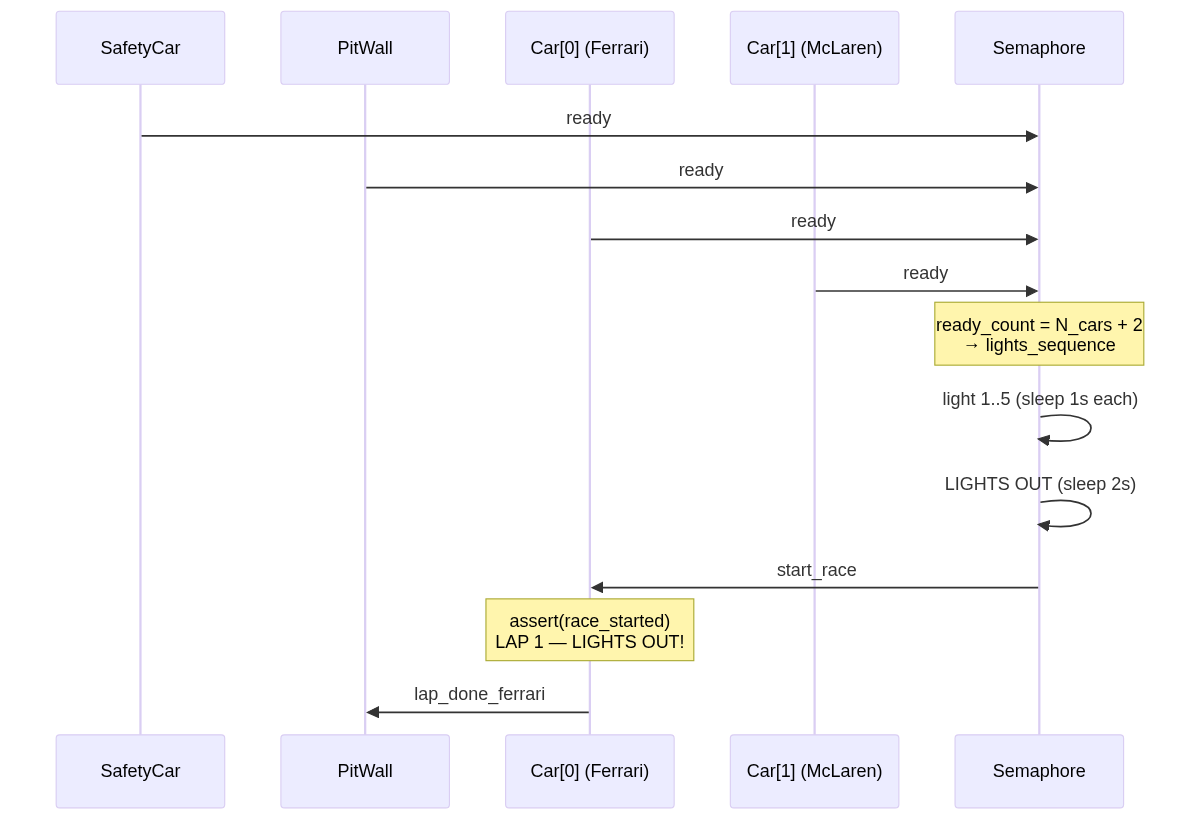
\includegraphics[width=\textwidth]{../../imgs/01_startup.png}
  \caption{Startup sequence: all agents register with the semaphore, which runs the lights
           sequence and fires \texttt{start\_race} to the first car.}
  \label{fig:seq_startup}
\end{figure}

\subsection{Lap Round-Robin}

\begin{figure}[H]
  \centering
  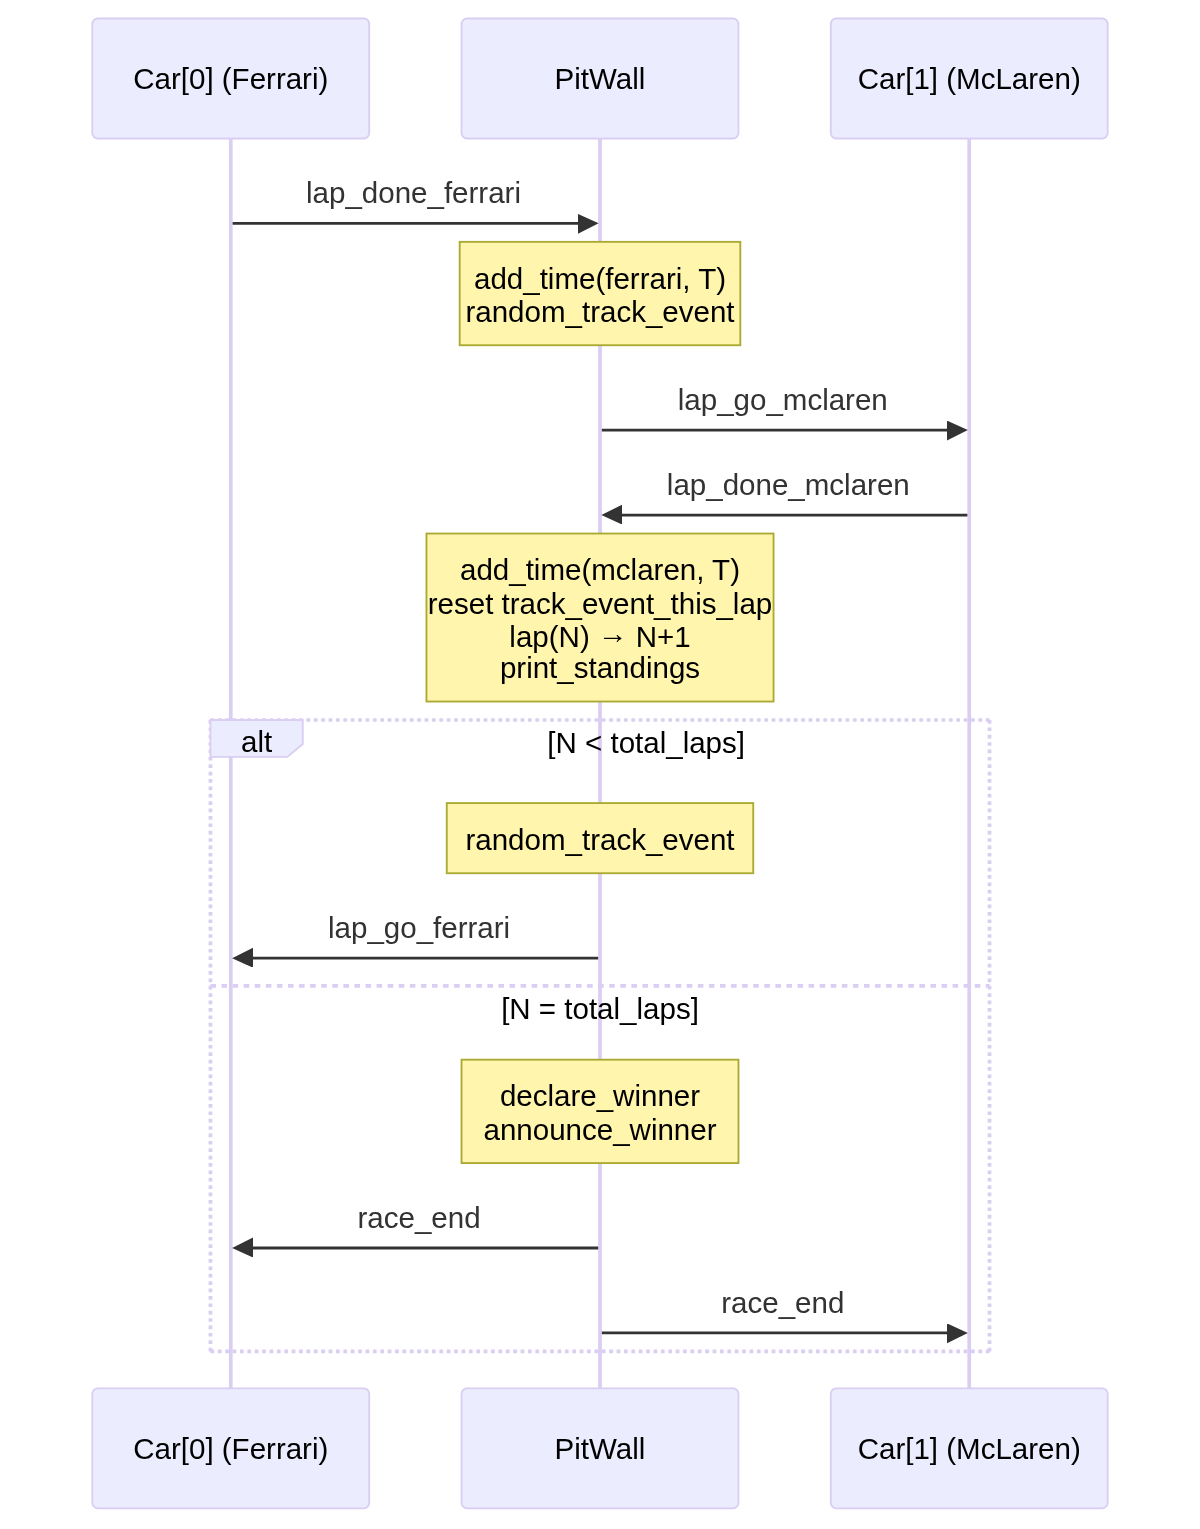
\includegraphics[width=\textwidth]{../../imgs/02_lap_roundrobin.png}
  \caption{Lap round-robin: the pit wall dispatches \texttt{lap\_go} tokens in order,
           accumulates lap times, and increments the lap counter after the last car.}
  \label{fig:seq_lap}
\end{figure}

\subsection{Safety Car Deployment}

\begin{figure}[H]
  \centering
  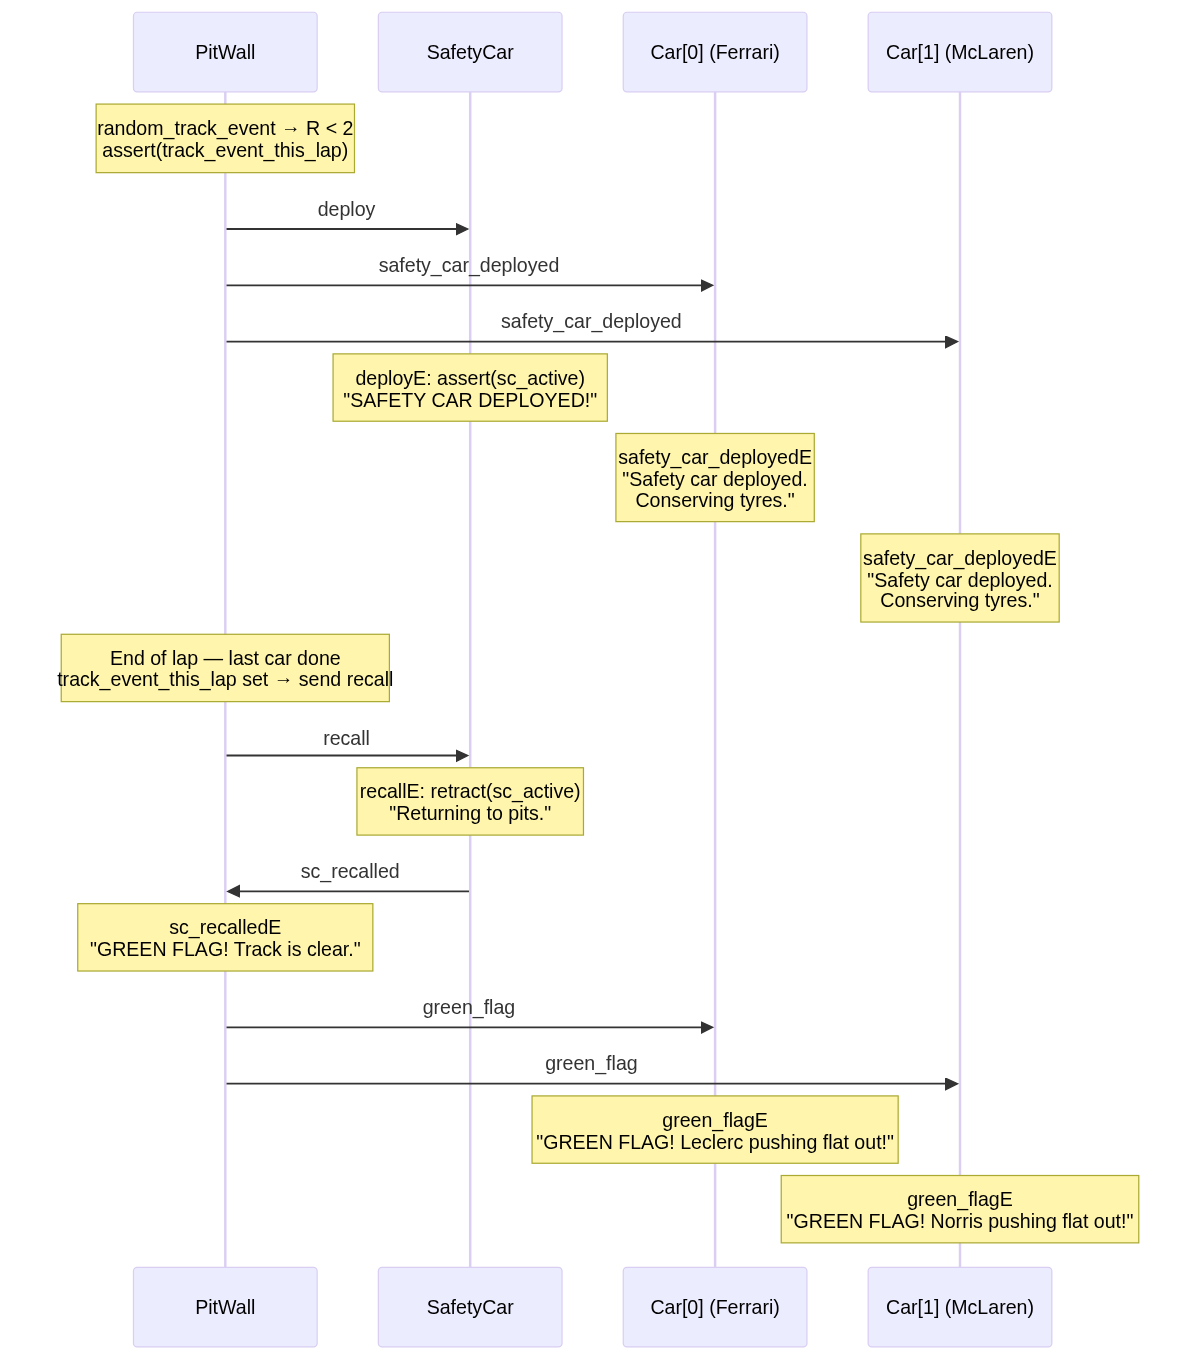
\includegraphics[width=\textwidth]{../../imgs/03_safety_car.png}
  \caption{Safety car chain: pit wall deploys the safety car and notifies all cars;
           at the end of the lap the safety car is recalled and the green flag is broadcast.}
  \label{fig:seq_sc}
\end{figure}

\subsection{Engine Failure (DNF)}

\begin{figure}[H]
  \centering
  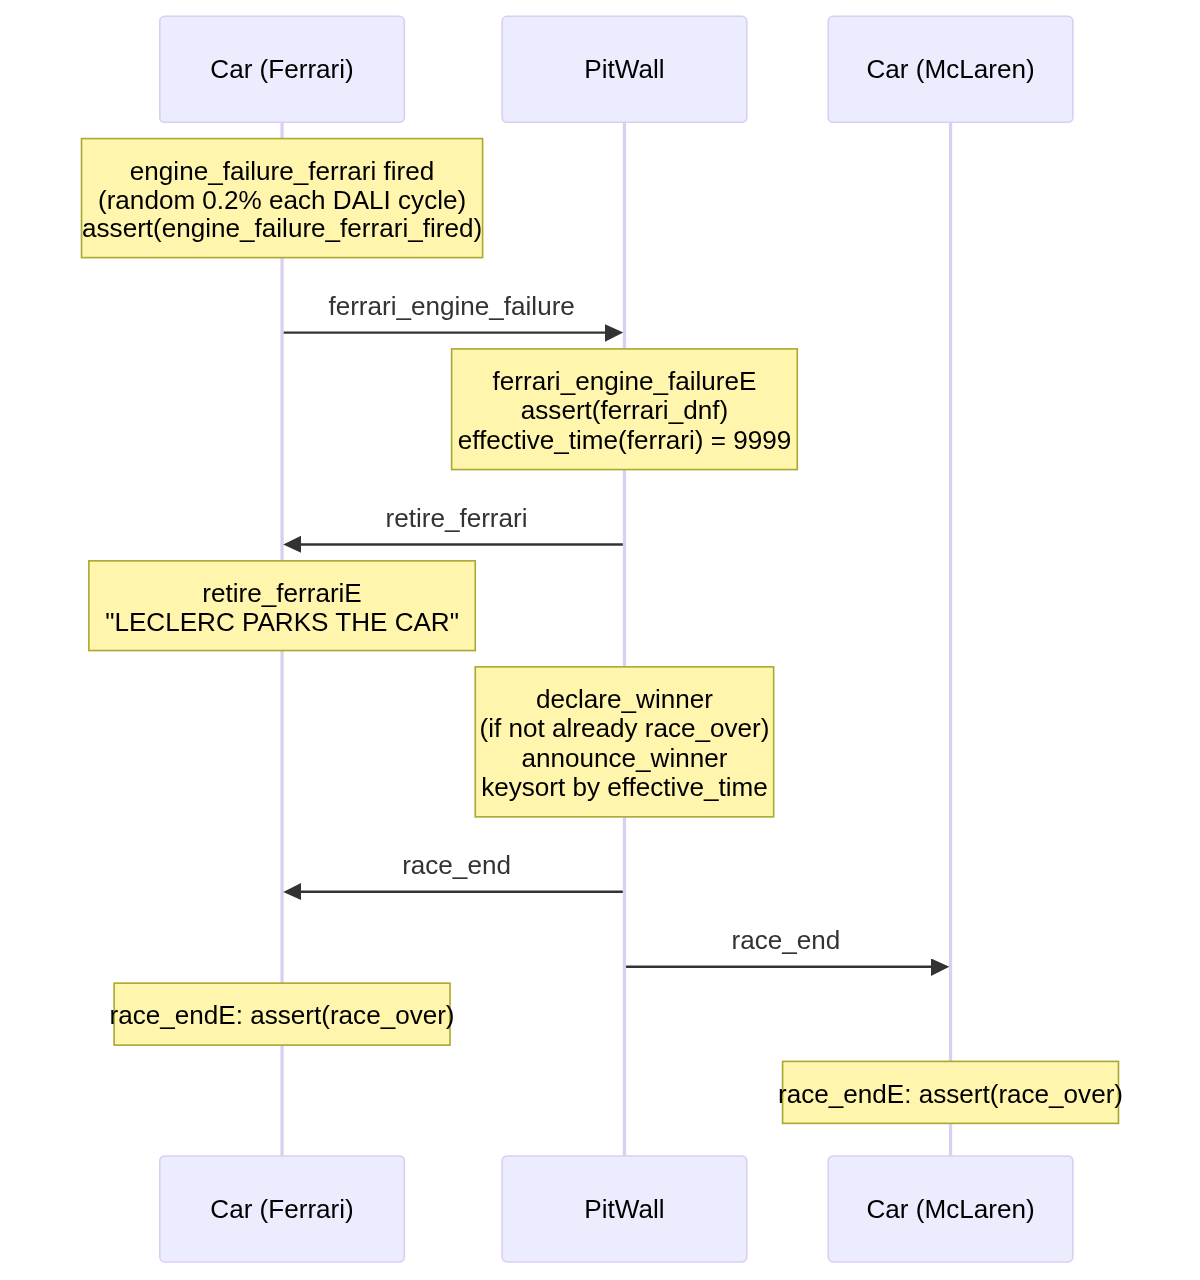
\includegraphics[width=\textwidth]{../../imgs/04_engine_failure.png}
  \caption{Engine failure: a car's internal event notifies the pit wall, which sets the
           DNF time, retires the car, and immediately calls \texttt{declare\_winner}.}
  \label{fig:seq_dnf}
\end{figure}

\subsection{Push Lap (Fastest-Lap Bonus)}

\begin{figure}[H]
  \centering
  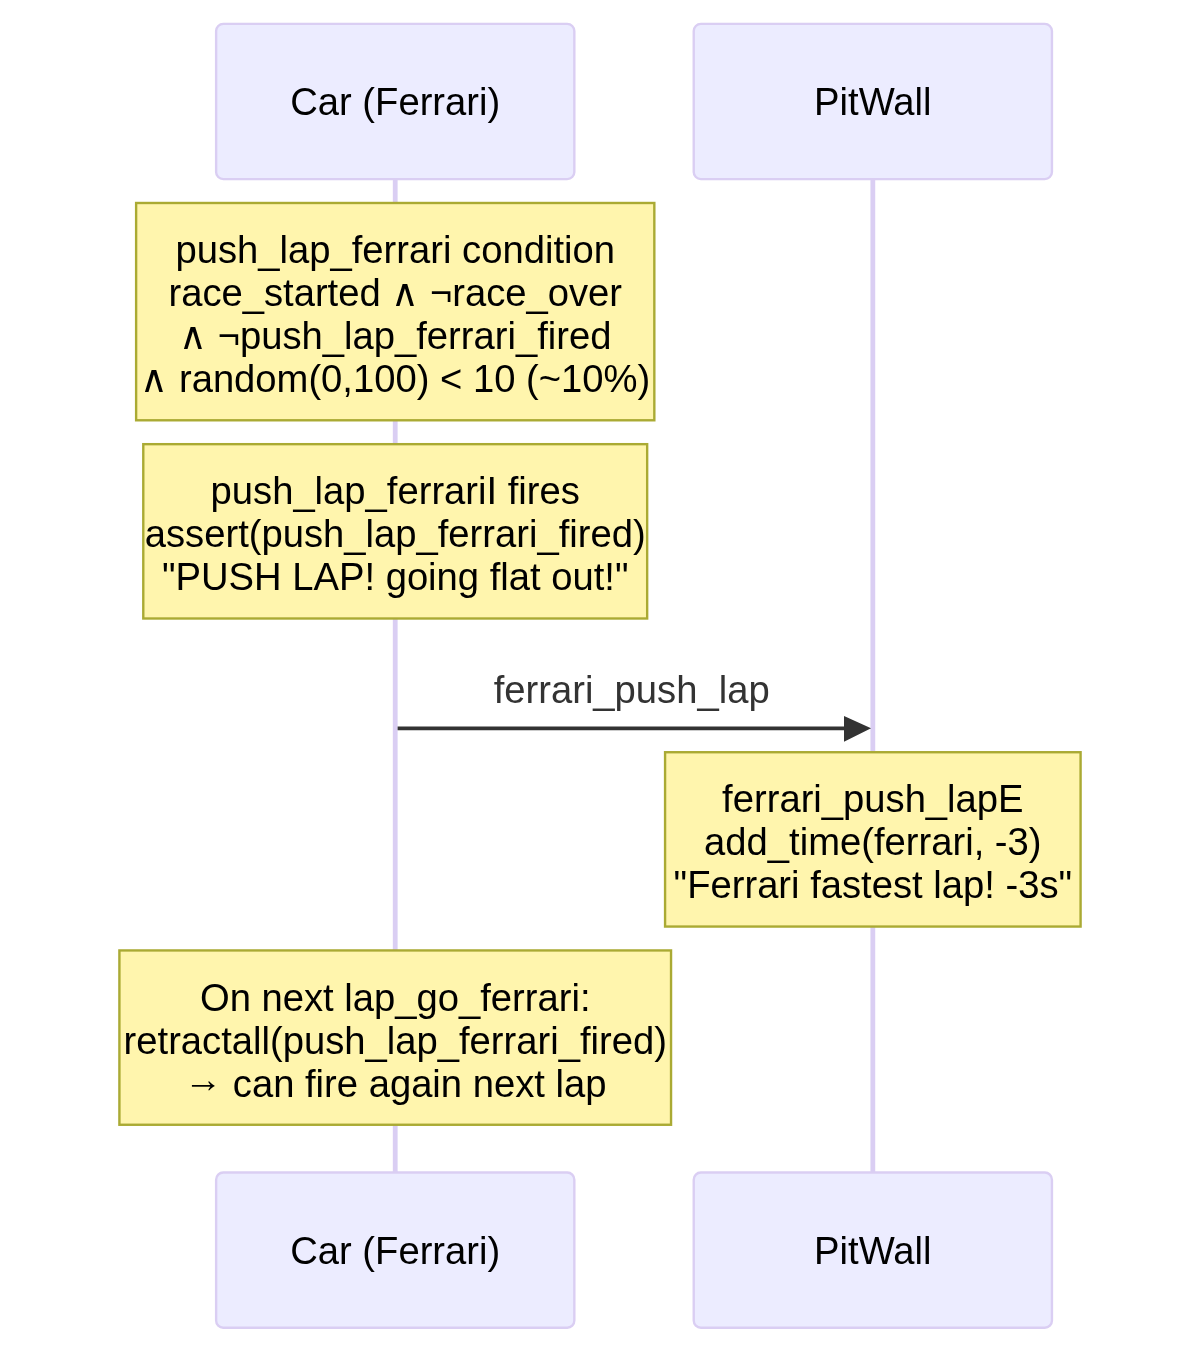
\includegraphics[width=\textwidth]{../../imgs/05_push_lap.png}
  \caption{Push lap: a car's internal event fires at most once per lap and notifies the
           pit wall, which deducts $3\,\text{s}$ from the car's accumulated time.}
  \label{fig:seq_push}
\end{figure}

% ================================================================
\section{Timing System}

The winner is the car with the lowest total accumulated time. Time is measured in seconds.

\begin{longtable}{@{} l r @{}}
\toprule
\textbf{Event} & \textbf{Time change} \\
\midrule
\endhead
Each lap      & $+\,\texttt{random}(60,\,90)$ seconds \\
Pit stop      & $+\,25\,\text{s}$ \\
Safety car (20\,\% per lap) & $+\,10\,\text{s}$ to \emph{all} cars \\
Heavy rain (20\,\% per lap) & $+\,5\,\text{s}$ to \emph{all} cars \\
Push lap (internal event, $\approx$10\,\%) & $-\,3\,\text{s}$ \\
Engine failure / DNF ($\approx$0.2\,\%) & $\texttt{time} = 9999\,\text{s}$ (race ends) \\
\bottomrule
\end{longtable}

\section{How to Run}

\subsection{Native (WSL / Linux)}

\begin{lstlisting}[language=bash, numbers=none]
cd DALI/Examples/f1_race
bash startmas.sh
\end{lstlisting}

\texttt{startmas.sh} performs the following steps:
\begin{enumerate}[leftmargin=2em]
  \item Kills any stale SICStus / tmux processes on port 3010.
  \item Runs \texttt{generate\_agents.py} to sync DALI files with \texttt{agents.json}.
  \item Builds agent binaries and launches all agents inside a single \texttt{tmux}
        session named \texttt{f1\_race}.
\end{enumerate}

\subsection{Web Dashboard}

In a second terminal:

\begin{lstlisting}[language=bash, numbers=none]
cd f1_race
bash ui/run.sh
\end{lstlisting}

\noindent
\texttt{run.sh} creates a local Python venv (\texttt{ui/.venv}) on the first run and
installs Flask automatically. Subsequent launches or skip \texttt{pip install} via a stamp
file (\texttt{.venv/.installed\_stamp}) and start it.

Open \url{http://localhost:5000} in a browser. The dashboard shows all agent panes
side-by-side with real-time auto-scrolling. If \texttt{agents.json} is modified while the
dashboard is open, it auto-detects the change within 5\,seconds and rebuilds the grid
without a page reload.

\begin{figure}[H]
  \centering
  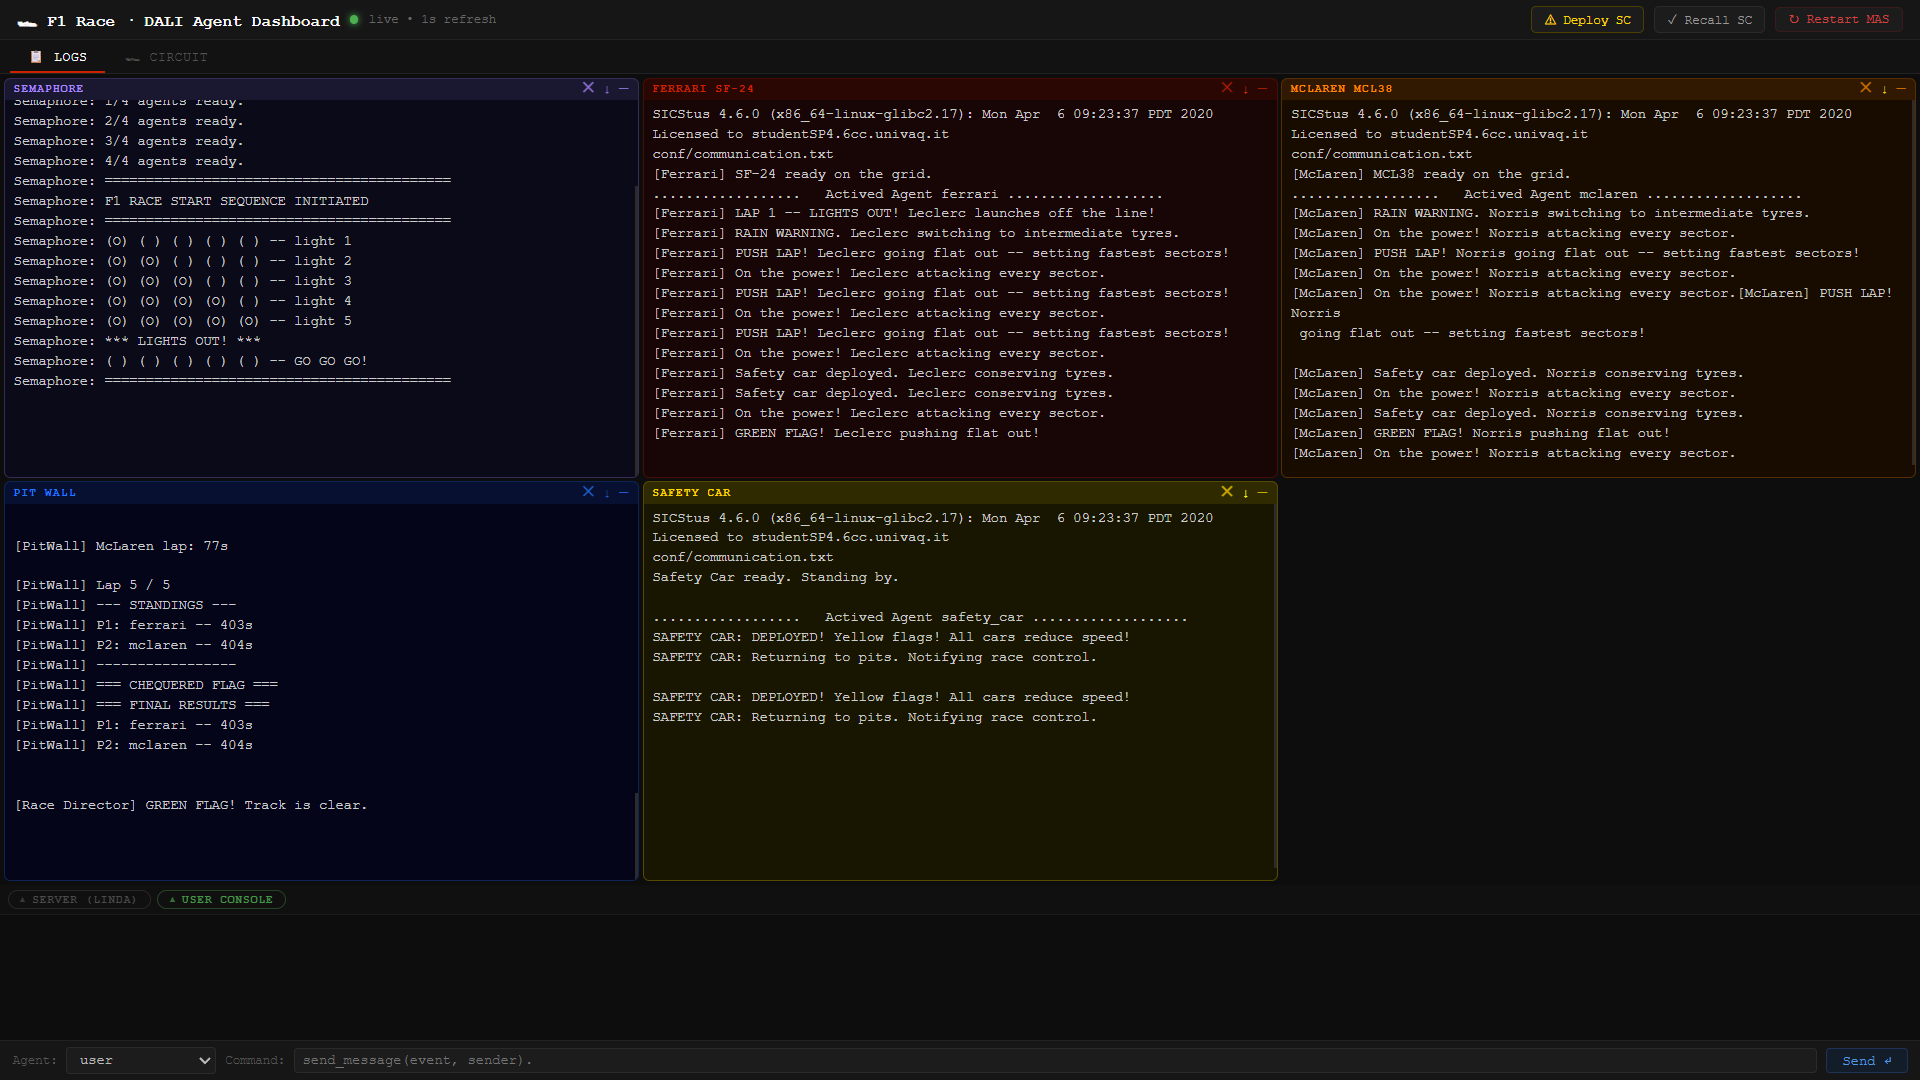
\includegraphics[width=\textwidth]{../../imgs/07_consoles.png}
  \caption{Web dashboard --- Logs tab: agent panes with real-time output, control buttons and command bar.}
  \label{fig:ui_consoles}
\end{figure}

\subsection{Dashboard Controls}

\begin{longtable}{@{} l p{9cm} @{}}
\toprule
\textbf{UI element} & \textbf{Function} \\
\midrule
\endhead
\textbf{Restart MAS}    & Kills SICStus + tmux session, reruns \texttt{startmas.sh} \\
\textbf{Deploy SC}      & Sends deploy message to safety car immediately \\
\textbf{Recall SC}      & Recalls the safety car \\
Agent / Command bar     & Sends an arbitrary Prolog command to any agent pane \\
Pin button ($\downarrow$) & Toggles auto-scroll for that pane \\
Clear button ($\times$)  & Clears pane output \\
Minimise button ($-$)   & Minimises pane to tray \\
\bottomrule
\end{longtable}

\begin{figure}[H]
  \centering
  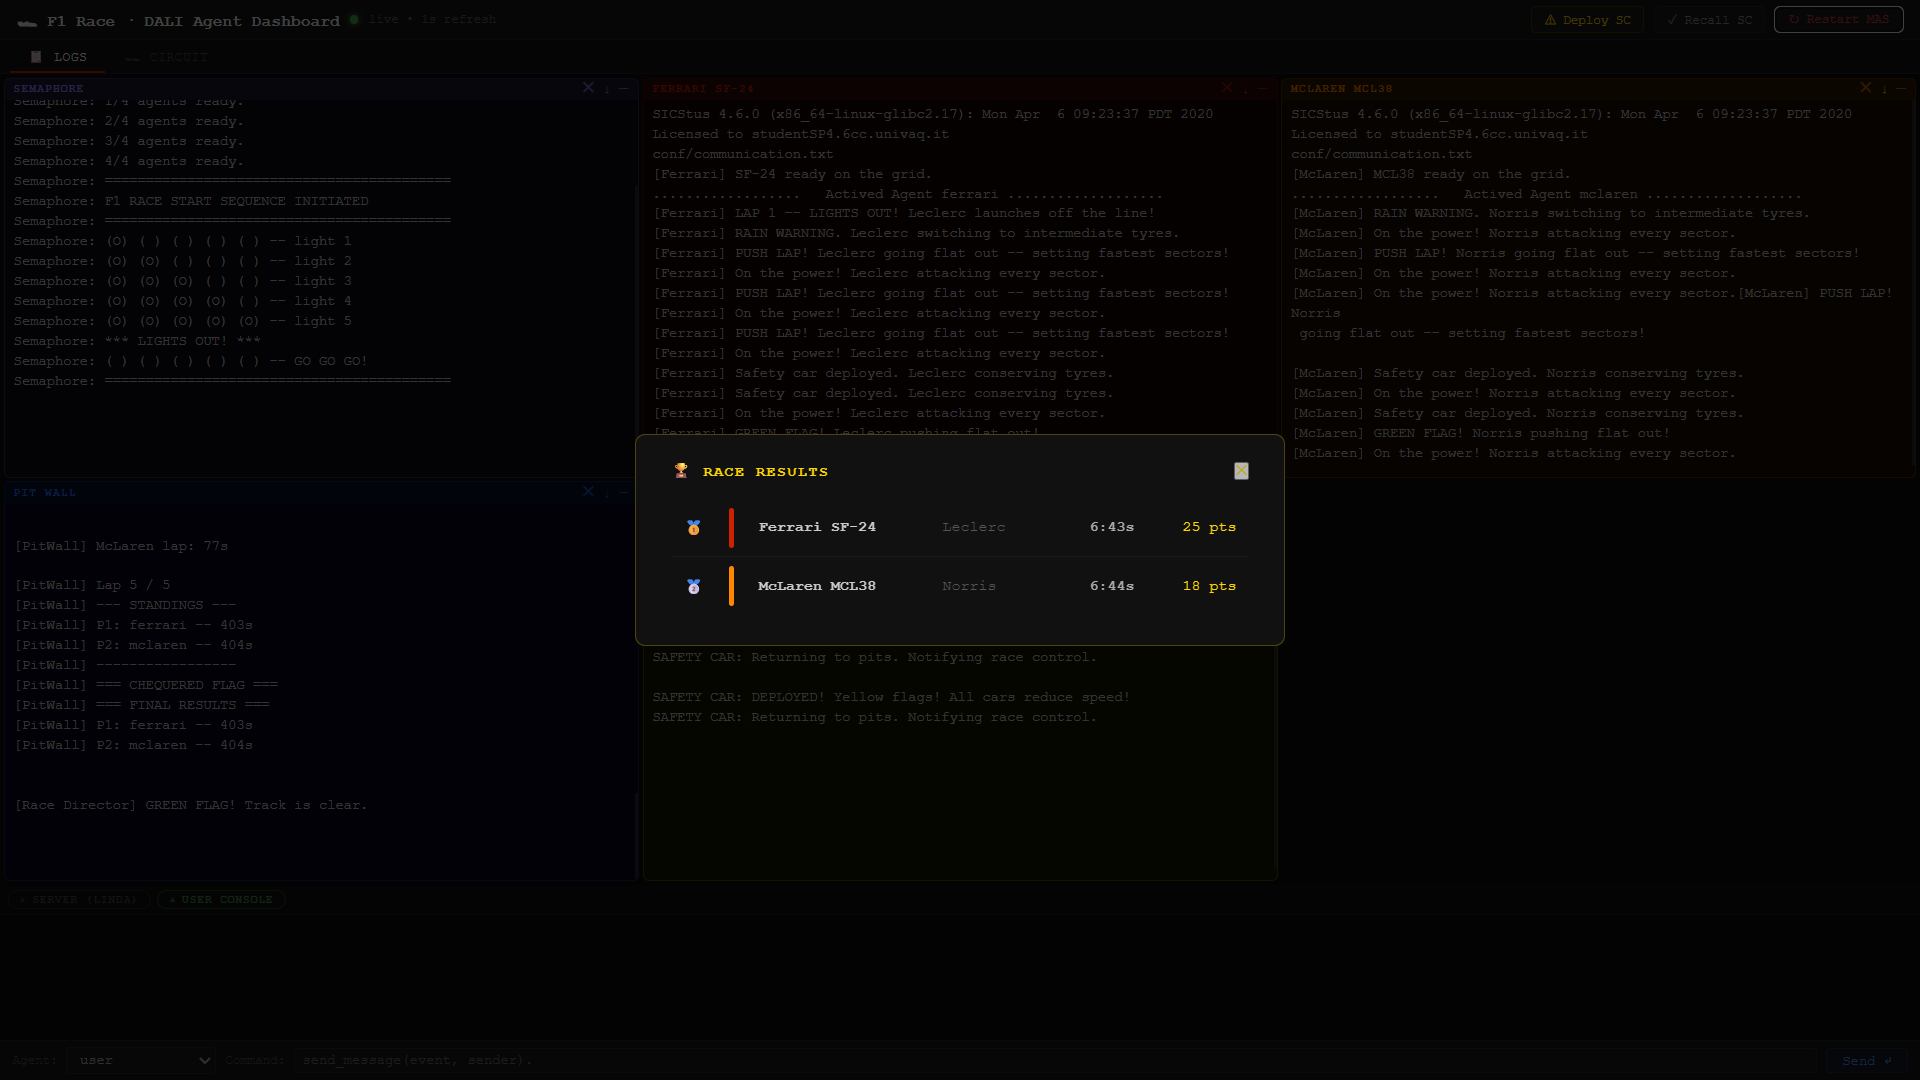
\includegraphics[width=\textwidth]{../../imgs/08_podium.png}
  \caption{Final podium modal displayed at race end, showing driver positions and total accumulated times.}
  \label{fig:ui_podium}
\end{figure}

\subsection{Circuit Tab}

The dashboard exposes two tabs selectable via the tab bar at the top of the page:

\begin{itemize}[leftmargin=2em]
  \item \textbf{Logs} --- the default view showing all agent panes side-by-side with
        real-time output.
  \item \textbf{Circuit} --- an animated canvas visualisation of the race circuit.
\end{itemize}

\noindent
Clicking a tab label switches the view instantly; no page reload is required. The
\texttt{Logs} tab remains fully active in the background (polling continues) while
the \texttt{Circuit} tab is open, so no agent output is ever lost.

The \textbf{Circuit tab} renders a Catmull-Rom spline track on an HTML5 Canvas and
animates each car along it in proportional time. Key features include:

\begin{itemize}[leftmargin=2em]
  \item \textbf{Start lights sequence} --- five red lights illuminate one per second
        before going out at race start, matching the semaphore agent's timing.
  \item \textbf{Car tokens} --- each car is drawn as a coloured dot with its team
        border glow, a lap-count badge, and a driver label. Position on track reflects
        the real fraction of the lap elapsed.
  \item \textbf{Pit-stop indicator} --- a car entering the pit lane is shown as
        stationary in the pit area for the duration of the stop.
  \item \textbf{Live sidebar} --- an always-visible leaderboard lists cars in current
        race order with their accumulated times, updated after every lap.
  \item \textbf{Final podium} --- once the race ends and all animations have played
        out, a modal overlay shows the final standings with positions and total times.
\end{itemize}

\begin{figure}[H]
  \centering
  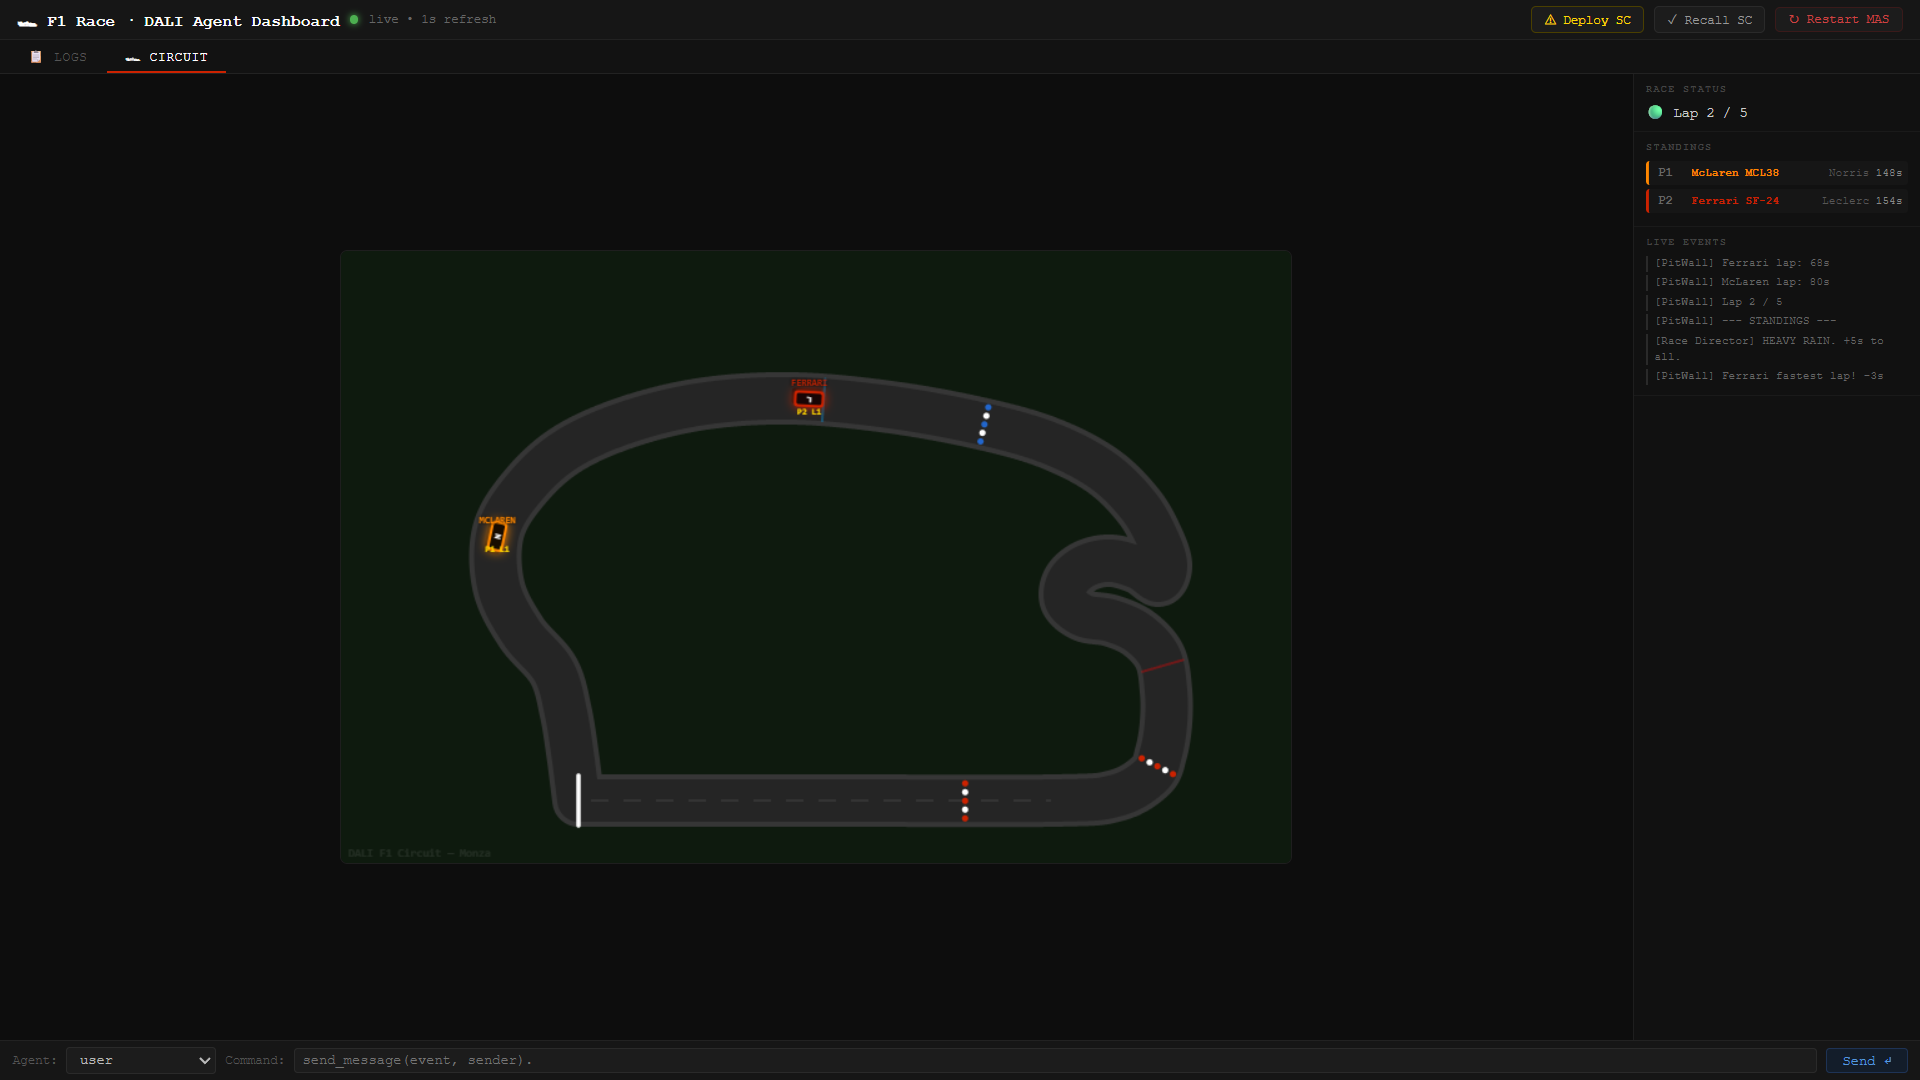
\includegraphics[width=\textwidth]{../../imgs/09_circuit.png}
  \caption{Web dashboard --- Circuit tab: animated Catmull-Rom track with car positions, start lights and live leaderboard sidebar.}
  \label{fig:ui_circuit}
\end{figure}

% ================================================================
\section{Docker Deployment}

\subsection{Architecture}

The Docker Compose setup runs two containers that share a tmux socket volume, allowing
the dashboard to read agent panes with zero modifications to the agent logic.

\begin{lstlisting}[language={}, numbers=none, frame=none, backgroundcolor=\color{white}]
+----------------------------------+   +------------------------------+
|  mas  (ubuntu:22.04)             |   |  ui  (python:3.11-slim)      |
|  startmas.sh -> tmux f1_race     |   |  dashboard.py (Flask :5000)  |
|  SICStus mounted from host (ro)  |   |  reads tmux panes via volume |
+----------------------------------+   +------------------------------+
                 tmux_sock volume (/tmp/tmux-shared)
\end{lstlisting}

\noindent
\textbf{Startup order} (managed by Docker healthchecks):
\begin{enumerate}[leftmargin=2em]
  \item \texttt{ui} starts immediately and is healthy once \texttt{/api/config} responds.
  \item \texttt{mas} waits for \texttt{ui} to be healthy, then runs \texttt{startmas.sh}.
\end{enumerate}

\subsection{Quickstart}

\begin{lstlisting}[language=bash, numbers=none]
cd DALI/Examples/f1_race

# 1. Auto-detect SICStus and write .env  (run once)
bash docker/setup.sh

# 2. Build and start
docker compose up --build -d

# 3. Open dashboard
open http://localhost:5000
\end{lstlisting}

\subsection{Environment Variables}

\begin{longtable}{@{} l l p{7cm} @{}}
\toprule
\textbf{Variable} & \textbf{Default} & \textbf{Description} \\
\midrule
\endhead
\texttt{SICSTUS\_PATH} & \texttt{/usr/local/sicstus4.6.0} & Host path to SICStus install, mounted read-only into the \texttt{mas} container \\
\bottomrule
\end{longtable}

% ================================================================
\section{DALI Syntax Reference}

The following table summarises all DALI syntax constructs used in this project.

\begin{longtable}{@{} l p{5.5cm} p{5.5cm} @{}}
\toprule
\textbf{Syntax} & \textbf{Meaning} & \textbf{Example} \\
\midrule
\endhead
\texttt{nameE:>~Body.}         & React to external event \texttt{name} & \texttt{start\_raceE:> write('Go!').} \\[4pt]
\texttt{nameI:>~Body.}         & Fire internal event when \texttt{name} holds & \texttt{push\_lap\_ferrariI:> send\_m(...).} \\[4pt]
\texttt{name :- Cond.}         & Condition for internal event \texttt{nameI} & \texttt{push\_lap\_ferrari :- race\_started, ...} \\[4pt]
\texttt{messageA(ag,\,msg)}    & Send message (top-level clause) & \texttt{messageA(pitwall, lap\_done).} \\[4pt]
\texttt{send\_m(ag,\,msg)}     & Send message (safe inside \texttt{if/3}) & \texttt{send\_m(safety\_car, deploy).} \\[4pt]
\texttt{random(Lo,\,Hi,\,R)}   & Random integer $\texttt{Lo} \le R < \texttt{Hi}$ & \texttt{random(0, 10, R).} \\[4pt]
\texttt{if(Cond,\,Then,\,Else)} & Conditional & \texttt{if(R < 5, act, true).} \\[4pt]
\texttt{\textbackslash+~Goal}  & Negation-as-failure & \texttt{\textbackslash+ race\_over} \\[4pt]
\texttt{:-~Goal.}              & Directive (runs at load time) & \texttt{:- write('Agent ready!').} \\[4pt]
\texttt{keysort(+P,\,-S)}      & Sort \texttt{Key-Value} pairs by key & \texttt{keysort([3-b,\,1-a],\,S).} \\
\bottomrule
\end{longtable}

% ================================================================
\section{Circuit Visualiser}

\subsection{Overview}

The dashboard contains two tabs switchable via a tab bar at the top of the page:

\begin{itemize}[leftmargin=2em]
  \item \textbf{Logs} --- the original side-by-side agent pane view.
  \item \textbf{Circuit} --- a Canvas-based animated race circuit that replays all
        lap events in proportional time, with start lights and a live sidebar.
\end{itemize}

\noindent
The tab system is managed by \texttt{switchTab(name)} in \texttt{app.js}, which calls
\texttt{circuitInit()} or \texttt{circuitDestroy()} from \texttt{circuit.js} to start
or stop the animation loop and API polling.

\subsection{\texttt{/api/race-state} Endpoint}

A dedicated Flask route \texttt{GET /api/race-state} parses the pitwall tmux pane via
regular expressions and returns a structured JSON object:

\begin{lstlisting}[language={}]
{
  "race_started": bool,
  "race_over":    bool,
  "safety_car":   bool,
  "current_lap":  int,
  "total_laps":   int,
  "cars": {
    "<id>": {
      "laps_completed": int,
      "lap_times":      [int, ...],   // seconds, one per completed lap
      "pit_stops":      int,
      "dnf":            bool,
      "total_time":     int,          // sum of lap_times
      "position":       int | null,   // last known P1/P2/... from standings
      "in_pit":         bool,
      "label":          str,
      "driver":         str,
      "team":           str,
      "color":          str,          // hex fill colour
      "border":         str           // hex glow colour
    }
  },
  "recent_events": [str, ...]  // last 8 notable pitwall lines
}
\end{lstlisting}

\noindent
The endpoint is polled every 2\,s by \texttt{circuit.js} while the circuit tab is active.
It applies purely textual regex parsing and never modifies agent state.

\subsection{Track Geometry}

The track is drawn on a fixed $760 \times 490$ px Canvas using a \emph{Catmull-Rom
closed spline} through 36 hand-tuned waypoints inspired by the Monza circuit layout.

\begin{enumerate}[leftmargin=2em]
  \item \textbf{Spline samples} --- \texttt{buildSplineSamples()} evaluates the
        Catmull-Rom formula at 80 steps per segment, producing a dense polyline.
  \item \textbf{Arc-length table} --- \texttt{buildArcTable()} computes cumulative arc
        lengths so that a normalised parameter $t \in [0,1]$ always maps to a
        \emph{uniform speed} position on the track, regardless of waypoint spacing.
  \item \textbf{Point lookup} --- \texttt{ptAtT(t)} binary-searches the arc table and
        linearly interpolates between the two nearest samples.
\end{enumerate}

\noindent
Visual layers drawn each frame (back to front):

\begin{enumerate}[leftmargin=2em]
  \item Dark green grass fill.
  \item Track outer-edge stripe (42\,px, dark grey).
  \item Asphalt surface (34\,px, darker grey).
  \item White dashed centre-line on the main straight.
  \item Start/Finish line (perpendicular white line at $t = 0$).
  \item Red/blue sector lines at $t = 0.34$ and $t = 0.67$.
  \item Red/white kerb dots at three apex positions.
  \item Safety-car yellow overlay (blinking, when active).
  \item Start-light panel (see Section~\ref{sec:startlights}).
  \item Car sprites and labels.
\end{enumerate}

\subsection{Animation State Machine}

\subsubsection{Event Queue}

Each car maintains a \emph{queue} of typed events:

\begin{longtable}{@{} l l p{7cm} @{}}
\toprule
\textbf{Type} & \textbf{Duration} & \textbf{Effect} \\
\midrule
\endhead
\texttt{lap} & $\texttt{timeS} \times 80$\,ms & Car travels from $t=0$ to $t=1$ along the track \\
\texttt{pit} & 4\,000\,ms & Car holds near the pit-lane entry ($t \approx 0.005$) \\
\texttt{dnf} & $\infty$ & Car stops and displays a DNF tombstone \\
\bottomrule
\end{longtable}

\noindent
The queue is only ever \emph{appended to} --- never rewound. On each API poll,
\texttt{updateCarAnim(data)} computes the difference between the API's
\texttt{laps\_completed} and the already-enqueued lap count and pushes only
\emph{new} events. This ensures the animation replay is idempotent.

\subsubsection{Chain Timing}

All events carry an absolute \texttt{startAt} timestamp so that the cumulative
display time faithfully reflects the real race time differences between cars:

\[
  \texttt{startAt}_i = \texttt{chainBase} + \sum_{j=0}^{i-1} \texttt{durationMs}_j
\]

\noindent
where \texttt{chainBase} is a shared wall-clock anchor assigned to all cars simultaneously.
Consequently a car with shorter lap times arrives at the S/F line earlier in
display-time on every lap, exactly mirroring the real race outcome.

\subsubsection{Animation Barrier and Synchronised Start}

Cars do not begin moving until an \emph{animation barrier} is set:

\begin{enumerate}[leftmargin=2em]
  \item \texttt{updateCarAnim()} is called on every API poll.
  \item After processing all cars, \texttt{\_trySetBarrier()} checks whether
        \emph{every} car has at least one lap enqueued.
  \item When all cars are ready, \texttt{\_animationBarrier} is set exactly once:
        $$\texttt{\_animationBarrier} = \texttt{\_raceStartedAt} + \texttt{LIGHTS\_OUT\_DELAY}$$
  \item \texttt{chainBase} is assigned to \texttt{\_animationBarrier} for every car
        in the same call, guaranteeing a perfectly synchronised start.
\end{enumerate}

\noindent
Without this barrier, cars whose lap data arrives in an earlier API poll would get an
earlier \texttt{chainBase} and start animated movement before other cars.

\subsection{Start Lights Sequence}\label{sec:startlights}

A standard F1 start-light panel is drawn over the track from the moment
\texttt{race\_started} becomes true (anchored to \texttt{\_raceStartedAt}):

\begin{longtable}{@{} l l @{}}
\toprule
\textbf{Elapsed time} & \textbf{State} \\
\midrule
\endhead
$0$--$1$\,s & 1 red light on \\
$1$--$2$\,s & 2 red lights on \\
$2$--$3$\,s & 3 red lights on \\
$3$--$4$\,s & 4 red lights on \\
$4$--$5$\,s & 5 red lights on \\
$5$--$5.2$\,s & Brief hold (all 5 on) \\
$5.2$\,s & Lights out --- cars begin moving; \emph{``LIGHTS OUT!''} flash \\
$5.2$--$7$\,s & Flash fades out \\
$> 7$\,s & Function returns immediately (zero overhead) \\
\bottomrule
\end{longtable}

\subsection{Leaderboard Gating}

In the Circuit tab the final leaderboard modal is intentionally delayed until the
animation has fully played out, so the visual outcome is not spoiled:

\begin{enumerate}[leftmargin=2em]
  \item \texttt{app.js} polls \texttt{/api/results}. If the result is available and the
        circuit tab is active but \texttt{circuitQueueDrained()} returns \texttt{false},
        the result is stored in \texttt{\_pendingLbResults} rather than shown.
  \item A 500\,ms \texttt{setInterval} in \texttt{app.js} watches
        \texttt{circuitQueueDrained()}; once it returns \texttt{true}
        (all car queues empty and all laps played), the saved results are displayed.
  \item \texttt{circuitQueueDrained()} (exported globally from \texttt{circuit.js})
        returns \texttt{true} only when every non-DNF car has an empty queue, no active
        event, and has played at least one lap.
\end{enumerate}

% ================================================================
\section{Shutdown}

\begin{lstlisting}[language=bash, numbers=none]
# Stop the MAS
tmux kill-session -t f1_race

# Stop the Flask dashboard
# Ctrl+C in the dashboard terminal

# Stop Docker
docker compose down
\end{lstlisting}

\end{document}
